% !TEX root = apresentacao.tex

% !TEX root = ./base.tex

%% abtex2-modelo-trabalho-academico.tex, v-1.9.5 laurocesar
%% Copyright 2012-2015 by abnTeX2 group at https://www.abntex.net.br
%%% This work may be distributed and/or modified under the
%% conditions of the LaTeX Project Public License, either version 1.3
%% of this license or (at your option) any later version.
%% The latest version of this license is in
%%  https://www.latex-project.org/lppl.txt
%% and version 1.3 or later is part of all distributions of LaTeX
%% version 2005/12/01 or later.
%%% This work has the LPPL maintenance status `maintained'.
%%
%% The Current Maintainer of this work is the abnTeX2 team, led
%% by Lauro César Araujo. Further information are available on
%% https://www.abntex.net.br/
%%% This work consists of the files abntex2-modelo-trabalho-academico.tex,
%% abntex2-modelo-include-comandos and abntex2-modelo-references.bib
%
% ------------------------------------------------------------------------
% ------------------------------------------------------------------------
% abnTeX2: Modelo de Trabalho Academico (tese de doutorado, dissertacao de
% mestrado e trabalhos monograficos em geral) em conformidade com
% ABNT NBR 14724:2011: Informacao e documentacao - Trabalhos academicos -
% Apresentacao
% ------------------------------------------------------------------------
% ------------------------------------------------------------------------

\documentclass[
  % -- opções da classe memoir --
  12pt,                 % tamanho da fonte
  openright,            % capítulos começam em pág ímpar (insere página vazia caso preciso)
  oneside,              % para impressão apenas no verso. Oposto a twoside
  a4paper,              % tamanho do papel.
  % twoside,            % para impressão em verso e anverso. Oposto a oneside
  % -- opções da classe abntex2 --
  chapter=TITLE,       % títulos de capítulos convertidos em letras maiúsculas
  %section=TITLE,       % títulos de seções convertidos em letras maiúsculas
  %subsection=TITLE,    % títulos de subseções convertidos em letras maiúsculas
  %subsubsection=TITLE, % títulos de subsubseções convertidos em letras maiúsculas
  % -- opções do pacote babel --
  english, % idioma adicional para hifenização
  french,  % idioma adicional para hifenização
  spanish, % idioma adicional para hifenização
  brazil   % o último idioma é o principal do documento
]{abntex2}

% --- Pacotes básicos ---
\usepackage{lmodern}        % Usa a fonte Latin Modern
\usepackage[T1]{fontenc}    % Selecao de codigos de fonte.
\usepackage[utf8]{inputenc} % Codificacao do documento (conversão automática dos acentos)
\usepackage{lastpage}       % Usado pela Ficha catalográfica
\usepackage{indentfirst}    % Indenta o primeiro parágrafo de cada seção.
\usepackage{color}          % Controle das cores
\usepackage{graphicx}       % Inclusão de gráficos
\usepackage{microtype}      % para melhorias de justificação
\usepackage{float}

% --- Pacotes adicionais, usados apenas no âmbito do Modelo Canônico do abnteX2 ---
\usepackage{lipsum}        % para geração de dummy text

% --- Pacotes de citações ---
\usepackage[brazilian,hyperpageref]{backref} % Paginas com as citações na bibl
\usepackage[alf]{abntex2cite}                % Citações padrão ABNT

% --- CONFIGURAÇÕES DE PACOTES ---

% ---  Configurações do pacote backref usado sem a opção hyperpageref de backref
\renewcommand{\backrefpagesname}{Citado na(s) página(s):~} % Texto padrão antes do número das páginas
\renewcommand{\backref}{}

% Define os textos da citação
\renewcommand*{\backrefalt}[4]{
  \ifcase#1     Nenhuma citação no texto.  \or{}
    Citado na página #2.  \else
    Citado #1 vezes nas páginas #2.  \fi}% ---
\setlength{\parindent}{1.3cm} % --- Espaçamentos entre linhas e parágrafos --- %
\setlength{\parskip}{0.2cm}  % Controle do espaçamento entre um parágrafo e outro: tente também \onelineskip
% Seleciona o idioma do documento (conforme pacotes do babel)
%\selectlanguage{english}
\selectlanguage{brazil}
\frenchspacing % Retira espaço extra obsoleto entre as frases.

\makeindex % --- compila o índice ---

% ADIÇÕES FEITAS POR MIM (João Vítor Fernandes Dias)

\usepackage{booktabs} % Necessários pra tabela
\usepackage{multirow} % Necessários pra tabela
\usepackage{animate}  % Necessário para animações
\usepackage{listings} % Necessário para código
\usepackage{caption}  % Colocar caption em códigos na parte de cima
\usepackage{adjustbox} % Adicionando Easter Eggs
\usepackage{ulem} % Adicionado para cortar texto
\usepackage{attachfile} % Anexando código ao PDF: alternativas: embedfile, navigator
\usepackage[table, dvipsnames]{xcolor} % Adding color to table line. Não tenho certeza para que o dvipsnames serve
\usepackage{subcaption} % Adicionar subfiguras

\attachfilesetup{
% color = {0 1 1}, % Cyan
color = {.05 .55 .18},
icon = Paperclip,
timezone = {-03'00'},
date={D:20240423173000000'00'},
mimetype = {application/x-rar-compressed},
% mimetype = {application/zip}
author = {Jo\~{a}o V\'{i}tor Fernandes Dias},
% author = {Joao Vitor Fernandes Dias},
% author = {João Vítor Fernandes Dias},
description = {Anexos da minha monografia},
subject = {Anexos da minha monografia. Mais especificamente, o seu código fonte.},
}

% --- Configurações de aparência do PDF final: alterando o aspecto da cor azul
\definecolor{hyperBlue}{HTML}{2905C3}

% Cores das tabelas em 2.02!7-resultados
\definecolor{myCellColor}{HTML}{79b8ff}
\definecolor{myRemoveLineColor}{HTML}{b31d28}
\definecolor{myAddLineColor}{HTML}{22863a}
\definecolor{hyperBlue}{HTML}{2905C3}

% Cores das Listings
\definecolor{codegreen}{HTML}{009900}
\definecolor{codegray}{HTML}{808080}
\definecolor{codepurple}{HTML}{9400D3}
\definecolor{backcolour}{HTML}{F2F2EB}

% Colore tabelas em 2.02!7-resultados
\newcommand{\altered}{\cellcolor{myCellColor}} % Define a cor desta célula
\newcommand{\removeLine}{\rowcolor{myRemoveLineColor}} % Define a cor da próxima linha
\newcommand{\addLine}{\rowcolor{myAddLineColor}} % Define a cor da próxima linha

% \captionsetup[lstlisting]{position=t}

\renewcommand{\lstlistingname}{Código}% Listing -> Código
\renewcommand{\lstlistlistingname}{Lista de \lstlistingname s} % List of Listings -> Lista de códigos

% Necessário para códigos bonitos

\lstdefinestyle{mystyle}{
  backgroundcolor=\color{backcolour},
  commentstyle=\color{codegreen},
  keywordstyle=\color{magenta},
  numberstyle=\tiny\color{codegray},
  stringstyle=\color{codepurple},
  basicstyle=\ttfamily\footnotesize,
  breakatwhitespace=false,
  breaklines=true,
  captionpos=b,
  keepspaces=true,
  numbers=left,
  numbersep=5pt,
  showspaces=false,
  showstringspaces=false,
  showtabs=false,
  tabsize=2
}

% numberbychapter=⟨true|false⟩ true % If true, and \thechapter exists, listings are numbered by chapter. Otherwise, they are numbered sequentially from the beginning of the document. This key can only be used before \begin{document}.

\lstset{style=mystyle}

\def\selfAuthor{Fonte: autoria própria} % Fonte padrão para figuras

% Figuras automaticamente centralizadas com fonte
\newenvironment{CenteredFigure}{\begin{figure}[htbp]\centering}{\end{figure}}
\newenvironment{MyCenteredFigure}{\begin{CenteredFigure}}{\legend{\selfAuthor}\end{CenteredFigure}}

\newenvironment{CenteredTable}{\begin{table}[htbp]\centering}{\end{table}} % Centered Tables

% Adicionar comando mais denso para adição da animação
\newcommand{\myAnimation}[1]{\includegraphics[scale=0.2]{files/img/2.02!5-desenvolvimento/2.02!5.1.4-sistema/Animacao/#1}}

% Coloring YAML: https://tex.stackexchange.com/questions/152829/how-can-i-highlight-yaml-code-in-a-pretty-way-with-listings

% \definecolor{commentColor}{HTML}{54A668}
% \definecolor{keyWordColor}{HTML}{569CD6}
% \definecolor{textColor}{HTML}{CE9178}

% \newcommand\YAMLcolonstyle{\color{commentColor}\mdseries}
% \newcommand\YAMLkeystyle{\color{keyWordColor}\bfseries}
% \newcommand\YAMLvaluestyle{\color{textColor}\mdseries}

\newcommand{\YAMLcolonstyle}{\color{red}\mdseries}
\newcommand{\YAMLkeystyle}{\color{black}\bfseries}
\newcommand{\YAMLvaluestyle}{\color{blue}\mdseries}

\makeatletter

% here is a macro expanding to the name of the language
% (handy if you decide to change it further down the road)
\newcommand\language@yaml{yaml}

\expandafter\expandafter\expandafter\lstdefinelanguage
\expandafter{\language@yaml}
{
keywords={true,false,null,y,n},
keywordstyle=\color{darkgray}\bfseries,
basicstyle=\YAMLkeystyle,                                 % assuming a key comes first
sensitive=false,
comment=[l]{\#},
morecomment=[s]{/*}{*/},
commentstyle=\color{purple}\ttfamily,
stringstyle=\YAMLvaluestyle\ttfamily,
moredelim=[l][\color{orange}]{\&},
moredelim=[l][\color{magenta}]{*},
moredelim=**[il][\YAMLcolonstyle{:}\YAMLvaluestyle]{:},   % switch to value style at :
morestring=[b]',
morestring=[b]",
literate =    {---}{{\ProcessThreeDashes}}3
{>}{{\textcolor{red}\textgreater}}1
{|}{{\textcolor{red}\textbar}}1
{\ -\ }{{\mdseries\ -\ }}3,
}

% switch to key style at EOL
\lst@AddToHook{EveryLine}{\ifx\lst@language\language@yaml\YAMLkeystyle\fi}
\makeatother

\newcommand\ProcessThreeDashes{\llap{\color{cyan}\mdseries-{-}-}}

% \newcommand{\importTeX}[1]{\include{files/tex/#1}} % Importar arquivos tex de forma mais enxuta % contra: perde os hiperlinks do vscode

\newcommand{\LinkToURL}[2]{\href{#1}{#2}\footnote{\url{#1}}}

% --- COMANDOS PARA CRIAR AS QUESTÕES DO FORMULÁRIO ---

\newcommand{\MyCheckbox}[2] {
  \item \CheckBox[name=#2, checkboxsymbol=\ding{53}]{ } #1
}

\newcommand{\FormInNewLine}[1]{
  \begin{description}
    \item[] #1
  \end{description}
}

\newcommand{\QuestionNameOptions}[3]{
  \item #1
  \FormInNewLine{\ChoiceMenu[print, combo, name=#2]{ }{#3}}
}

\newcommand{\ChoiceMenuPeriodos}[2]{
  \QuestionNameOptions{#1}{#2}{ 0, 1, 2, 3, 4, 5, 6, 7, 8, 9, 10 }
}

\newcommand{\ChoiceMenuSNO}[2]{
  \QuestionNameOptions{#1}{#2}{1. Sim, 2. Não, 3. Outro }
}

\newcommand{\ChoiceMenuDdNcC}[2]{
  \QuestionNameOptions{#1}{#2}
  {
    1. Discordo completamente,
    2. Discordo parcialmente,
    3. Não tenho preferência,
    4. Concordo parcialmente,
    5. Concordo completamente
  }
}

% Seguindo a NBR 6023
\makeatletter
\@ifpackageloaded{url}{%
  \addtociteoptionlist{abnt-url-package=url}
  \def\UrlLeft{}
  \def\UrlRight{}
  \urlstyle{same}}
\makeatother
% Seguindo a NBR 6023

% --- DEFININDO LINKS USADOS AO LONGO DO DOCUMENTO ---

% 2.01!1-introducao
\def\LinkDrawio{https://www.drawio.com} % 2.02!3-organizacao; 2.02!4-modelagem
\def\LinkMermaid{https://mermaid.js.org}

% 2.02!3-organizacao
\def\LinkEstatuto{https://uenf.br/UENF_ARQUIVOS/Downloads/REITORIA_1360_1101117875.pdf}
\def\LinkSiteUENF{https://uenf.br/portal}
\def\LinkCCH{https://uenf.br/cch}
\def\LinkCCT{https://uenf.br/cct}
\def\LinkCBB{https://uenf.br/cbb}
\def\LinkCCTA{https://uenf.br/ccta}
\def\LinkLaboratorios{https://uenf.br/cct/administracao/laboratorios}
\def\LinkLAMET{https://uenf.br/cct/lamet}
\def\LinkLCFIS{https://uenf.br/cct/lcfis}
\def\LinkLECIV{https://uenf.br/cct/leciv}
\def\LinkLCQUI{https://uenf.br/cct/lcqui}
\def\LinkLAMAV{https://uenf.br/cct/lamav}
\def\LinkLCMAT{https://uenf.br/cct/lcmat}
\def\LinkLEPROD{https://uenf.br/cct/leprod}
\def\LinkLENEP{https://uenf.br/cct/lenep}
\def\LinkLicMat{https://uenf.br/posgraduacao/licenciatura-matematica}
\def\LinkSiteCCUENF{https://cc.uenf.br}
\def\LinkLCMATPósGraduação{https://uenf.br/posgraduacao/matematica/apresentacao}
\def\LinkUENFPósGraduações{https://uenf.br/posgraduacao/programas/pos-graduacao}
\def\LinkProfMat{https://profmat-sbm.org.br}
\def\LinkDistribuiçãoDeSalas{https://uenf.br/cct/secretaria-academica/distribuicao-das-salas-de-aula-do-cct}
\def\LinkRabbitMQ{https://rabbitmq.com}
\def\LinkGitLab{https://about.gitlab.com}

% 2.02!5-desenvolvimento
\def\LinkPython{https://www.python.org}
\def\LinkProjetoDemanda{https://github.com/jvfd3/university_demand}
\def\LinkPDFMiner{https://pypi.org/project/pdfminer}
\def\LinkLGPD{https://www.planalto.gov.br/ccivil_03/_ato2015-2018/2018/lei/l13709.htm}
\def\LinkLGPDEstudoTécnico{https://www.gov.br/anpd/pt-br/assuntos/noticias/sei_00261-000810_2022_17.pdf}
\def\LinkFigma{https://www.figma.com}
\def\LinkVelcro{https://en.wikipedia.org/wiki/Hook-and-loop_fastener}
\def\LinkGitHubProjects{https://docs.github.com/pt/issues/planning-and-tracking-with-projects}
\def\LinkJSONBin{https://jsonbin.io}
\def\LinkMySQL{https://www.mysql.com}
\def\LinkAxios{https://axios-http.com}
\def\LinkExpress{https://expressjs.com}
\def\LinkNodeJS{https://nodejs.org}
\def\LinkReactRouter{https://reactrouter.com}
\def\LinkReactSelect{https://react-select.com}
\def\LinkAcademicoUENF{https://academico.uenf.br}

% 2.02!6-experimentos
\def\LinkLiveSplit{https://livesplit.org}
\def\LinkNotebook{https://www.asus.com/br/supportonly/x571gt/helpdesk_manual}

% 3.03#-apendice
\def\LinkCodigoFonteSistema{https://github.com/jvfd3/timetabling-UENF}
\def\LinkAdobeReader{https://get.adobe.com/br/reader}
\def\LinkDisciplinas{https://github.com/UENF-Organizacao-de-Disciplinas}
\def\LinkCodigoFonteMonografia{https://github.com/UENF-Organizacao-de-Disciplinas/INF01131-Monografia}


% % --- Informações de dados para CAPA e FOLHA DE ROSTO --- %

\autor{João Vítor Fernandes Dias}
\titulo{\textit{Timetabling Problem}: desafios no desenvolvimento de um sistema de decisão voltado ao problema de organização de tabela de horários no ensino superior}
\local{Campos dos Goytacazes, RJ}
\data{\today}

\def\orientadorTCC{Fermín Alfredo Tang Montané}

\preambulo{Trabalho de Conclusão de Curso apresentado ao Curso de Graduação em Ciência da Computação da Universidade Estadual do Norte Fluminense Darcy Ribeiro, sob orientação do Prof. Dr. \orientadorTCC}
% \instituicao{Universidade Estadual do Norte Fluminense Darcy Ribeiro \par Ciência da Computação \par Metodologia de Pesquisa}
\orientador{\orientadorTCC}
\tipotrabalho{Projeto de Pesquisa}
%\coorientador{Equipe \abnTeX}
% O preambulo deve conter o tipo do trabalho, o objetivo, o nome da instituição e a área de concentração
% ---

% ---
% Configurações de aparência do PDF final
% alterando o aspecto da cor azul
\definecolor{blue}{RGB}{41,5,195}

% informações do PDF
\makeatletter
\hypersetup{
  %pagebackref=true,
  pdftitle={\@title},
  pdfauthor={\@author},
  pdfsubject={\imprimirpreambulo},
  pdfcreator={LaTeX with abnTeX2},
  pdfkeywords={abnt}{latex}{abntex}{abntex2}{trabalho acadêmico},
  % pdfkeywords={Tabela de horários}{Agendamento de aulas universitárias}{Heurísticas}{Programação Inteira}{Representação do Conhecimento}{Interação Homem Computador},
  colorlinks=true,           % false: boxed links; true: colored links
  linkcolor=blue,            % color of internal links
  citecolor=blue,            % color of links to bibliography
  filecolor=magenta,         % color of file links
  urlcolor=blue,
  bookmarksdepth=4
}
\makeatother


\begin{document} % --- Início do documento ---
\pretextual{} % --- INÍCIO DOS ELEMENTOS PRÉ-TEXTUAIS ---

% \imprimircapa{} % Capa
% \imprimirfolhaderosto{} % Folha de rosto (o * indica que haverá a ficha bibliográfica)

% % # Testando LaTeX

\chapter{Teste RGB}

Teste pra saber de que forma que o filtro de cor cinza no vscode tá afetando a visualização das minhas imagens.

\begin{MyCenteredFigure} \caption{Teste de RGB}
  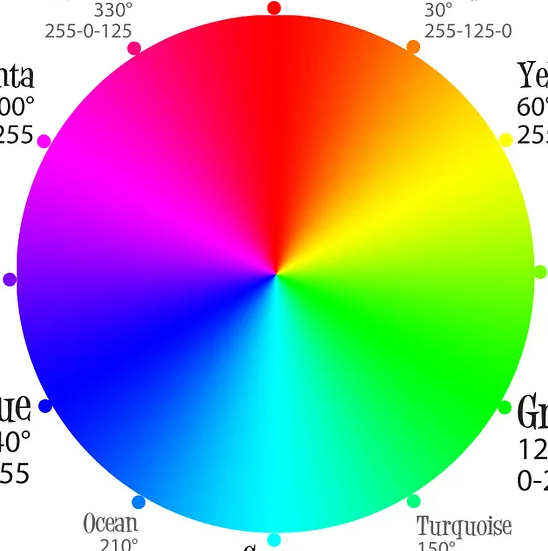
\includegraphics[width=0.5\textwidth]{files/img/unused/teste RGB.png}
\end{MyCenteredFigure}

\chapter{Embedding}

ATACHING

% \attachfile{files/codigos/ATTACH.txt}

% test \textattachfile[color=1 0 0]{files/codigos/ATTACH.txt}{Texto 1}

% test \textattachfile[color=0 1 1]{files/codigos/ATTACH.txt}{Texto 2}

% \textattachfile[]{files/codigos/CodigoFonteLaTeX.rar.RemovaEstaPartaParaAcessarOCodigo}{Texto 3}

% EMBEDING

% \embedfile[desc={DECRICAO}]{files/codigos/EMBED.txt}

% \embedfile[desc={DECRICAO2}]{files/codigos/CódigoFonte.rar}

% \embedfile[desc={DECRICAO3}]{files/codigos/CódigoFonte.rar.RemovaEstaPartaParaAcessarOCódigo}

% \embeddedfile{alias}{files/codigos/EMBED2.txt}

% \openfilelink{files/codigos/EMBED2.txt}{Clique aqui para abrir o arquivo}


\chapter{Easter Egg}

% \begin{MyCenteredFigure}
%   \caption{Teste de Easter Egg}
%   
\includegraphics[width=0.5\textwidth]{files/img/unused/teste}

%   \adjustbox{trim={.25\width} {.25\height} {.25\width} {.25\height},clip}{
\includegraphics[width=0.5\textwidth]{files/img/unused/teste}}
% \end{MyCenteredFigure}

\chapter{Build}

1

ABCDEFGHIJKLMNOPQRSTUVWXYZ

2


% Ficha catalográfica

% % !TEX root = base.tex
% --- Inserir folha de aprovação --- %

% Isto é um exemplo de Folha de aprovação, elemento obrigatório da NBR
% 14724/2011 (seção 4.2.1.3). Você pode utilizar este modelo até a aprovação
% do trabalho. Após isso, substitua todo o conteúdo deste arquivo por uma
% imagem da página assinada pela banca com o comando abaixo:
% \includepdf{folhadeaprovacao_final.pdf}
\begin{folhadeaprovacao}

  \begin{center}
    {\ABNTEXchapterfont\large\imprimirautor}

    \vspace*{\fill}\vspace*{\fill}
    \begin{center}
      \ABNTEXchapterfont\bfseries\Large\imprimirtitulo
    \end{center}
    \vspace*{\fill}

    \hspace{.45\textwidth}
    \begin{minipage}{.5\textwidth}
      \imprimirpreambulo
    \end{minipage}
    \vspace*{\fill}
  \end{center}

  Trabalho aprovado. \imprimirlocal, 2 de julho de 2024:

  % \assinatura{\textbf{Prof. Dr. \imprimirorientador} \\ Orientador}
  \assinatura{\textbf{Prof. Dr. Fermín A. Tang Montané} \\ Orientador}
  \assinatura{\textbf{Prof. Dr. Luis Antonio Rivera Escriba} \\ Membro da banca}
  \assinatura{\textbf{Profa. Dra. Annabell Del Real Tamariz} \\ Membro da banca}
  %\assinatura{\textbf{Professor} \\ Convidado 3}
  %\assinatura{\textbf{Professor} \\ Convidado 4}

  \begin{center}
    \vspace*{0.5cm}
    {\large\imprimirlocal}
    \par
    {\large\imprimirdata}
    \vspace*{1cm}
  \end{center}

\end{folhadeaprovacao}

% \chapter*{Banca}

% Por enquanto, a banca que eu tenho em mente é composta por:

% \begin{enumerate}
%   \item Fermín Alfredo Tang Montané (Orientador)
%   \item Annabell del Real Tamariz (Ex Chefe do Laboratório de Matemática)
%   \item Oscar Alfredo Paz La Torre (Ex Diretor do CCT)
%   \item Luiz Humberto Guillermo Felipe (Chefe do Laboratório de Matemática)
%   \item Márcia Diretora CCT (Diretora do CCT)
% \end{enumerate}

% Conforme resolução 004/2007 do COLAC, artigo 9 e parágrafo 1, a banca examinadora deverá ter a seguinte composição:
% (i) o Professor Orientador e/ou Co-orientador do aluno, que presidirá os trabalhos,
% (ii) um membro indicado, de comum acordo, pelo estudante e seu Professor Orientador ou Co-Orientador e
% (iii) um membro indicado pelo Colegiado do Curso. Em caráter excepcional, um dos três avaliadores poderá ser um Mestre ou doutorando ou pós doutorando que tenha formação compatível com o tema da monografia. Além dos membros titulares, deverá ser indicado um membro suplente. A composição da banca deverá ser aprovada pelo Colegiado do Curso, dando preferência para que o presidente seja doutor. Quando o orientador ou co-orientador estiver impossibilitado de estar presente na banca examinadora, o coordenador do Curso poderá representá-lo, desde que seja requerido por escrito e antecipadamente pelo orientador do aluno.

% \begin{dedicatoria}
  \vspace*{\fill}
  \centering
  \noindent

  Primariamente eu dedico este trabalho a todos aqueles que me apoiaram, incentivaram e cobraram pela conclusão do meu TCC.

  Dedico este trabalho àqueles que vieram antes de mim, Sânya e Ricardo, que inicialmente pesquisaram e desenvolveram seus trabalhos sobre o mesmo tema.

  Dedico ao atual coordenador de Ciência da Computação na UENF, o Prof. Dr. Fermín Alfredo Tang Montané, que me deu a oportunidade de trabalhar com ele desde o início da minha graduação. E que esteve disponível a mim e aos alunos de computação em seus momentos de necessidade.

  Dedico a UENF, ao CCT e ao Curso de Ciência da Computação, que me guiaram na jornada de aprendizado e crescimento acadêmico.

  Mas principalmente dedico a todos os futuros alunos e pesquisadores, que inconformados com o \textit{status quo}, buscam sempre melhorar a si mesmos e ao mundo ao seu redor.

  \vspace*{\fill}
\end{dedicatoria}
% \begin{agradecimentos}

  Agradeço aos meus pais que se dedicaram para que eu pudesse estar cursando esta graduação, assim podendo completar mais uma etapa da minha vida. Sem o apoio, conselhos, carinho e amor, nada disso seria possível. Sou eternamente grato por tudo que vocês fazem e sempre fizeram para que minha vida fosse especial.

  Agradeço aos meus amigos e colegas de curso que compartilharam comigo bons momentos, risadas e refeições no RU. Em especial, aos meus grandes amigos Daniel Brito e José Lucio, que unidos pela Iniciação Científica e pela progressão contínua, seguimos juntos até o fim, também aos meus amigos João Víttor e Adriano, que entraram comigo no curso e que, apesar dos percalços, seguem sendo grandes companhias pra vida.

  Agradeço ao meu orientador, Prof. Dr. Fermín Alfredo Tang Montané, que se dispôs a me ouvir reclamar e propor ideias. Que se dispôs a me orientar mesmo que em suas férias, e que sempre esteve disponível para me ajudar.

\end{agradecimentos}
% \begin{epigrafe}
  \vspace*{\fill}
  \begin{flushright}
    \textit{``Quando você não sabe alguma coisa,\\
      procura quem sabe e pergunta\\
      pra não fazer feio, nem passar vergonha.\\
      Vovô Nando, 01/12/2023}
  \end{flushright}
\end{epigrafe}
% % resumo em português
\setlength{\absparsep}{18pt} % ajusta o espaçamento dos parágrafos do resumo
\begin{resumo}

  Este artigo visa apresentar uma análise da situação em que atualmente se encontra a criação de grades horárias na Universidade Estadual do Norte Fluminense, bem como apontar seus maiores problemas e desenvolver um sistema de decisão capaz de auxiliar diversos centros e laboratórios no desenvolvimento de suas grades horárias, buscando a otimização do uso de salas e redução dos conflitos existentes entre demandas de diferentes alunos por matérias.

  \textbf{Palavras-chave}: tabela de horários. agendamento de aulas universitárias. heurísticas. representação do conhecimento. interação humano-computador.

  % Resumo

  % Segundo a ABNT (2003, 3.1-3.2), o resumo deve ressaltar o objetivo, o método, os resultados e as conclusões do documento. A ordem e a extensão destes itens dependem do tipo de resumo (informativo ou indicativo) e do tratamento que cada item recebe no documento original. O resumo deve ser precedido da referência do documento, com exceção do resumo inserido no próprio documento. (. . . ) As palavras-chave devem figurar logo abaixo do resumo, antecedidas da expressão Palavras-chave:, separadas entre si por ponto e finalizadas também por ponto.

  % Palavras-chave: latex. abntex. editoração de texto.

\end{resumo}

% % resumo em inglês
\begin{resumo}[Abstract]
  \begin{otherlanguage*}{english}

    Esta monografia apresenta um estudo sobre a criação de grades horárias em universidades, com foco na Universidade Estadual do Norte Fluminense, e o desenvolvimento de um sistema de suporte à decisão para a criação de grades horárias. Este processo é complexo e envolve diversos fatores, como a disponibilidade de salas e professores, a quantidade de alunos e a demanda por disciplinas. Como uma das maiores dificuldades no ramo acadêmico da criação de grades horárias é a modelagem do problema, este trabalho se propõe a estruturar as informações referentes à instituição estudada através de pesquisas e entrevistas. A partir disso, foi possível identificar a sequência de criação das grades e as restrições impostas pela instituição, podendo assim propor um sistema que auxilie o processe. Para tanto, o sistema foi desenvolvido utilizando JavaScript e a biblioteca React, sendo hospedado no GitHub Pages e utilizando da Amazon Web Services para a execução de seu \textit{backend} e armazenamento de dados. Suas funcionalidades incluem as funcionalidades CRUD (criar, ler, atualizar e deletar) de professores, disciplinas, salas, alunos, turmas e horários, a criação automatizada de uma grade horária inicial para o curso de Ciência da Computação da UENF, a visualização de conflitos dentre os recursos alocados e a análise história dos dados armazenados no sistema.

    This monograph presents a study on the creation of timetables in universities, focusing on the Universidade Estadual do Norte Fluminense, and the development of a decision support system for the creation of timetables. This process is complex and involves several factors, such as the availability of classrooms and teachers, the number of students and the demand for disciplines. As one of the greatest difficulties in the academic field of creating timetables is the modeling of the problem, this work proposes to structure the information regarding the institution studied through research and interviews. From this, it was possible to identify the sequence of creating the timetables and the restrictions imposed by the institution, thus being able to propose a system that assists the process. For this, the system was developed using JavaScript and the React library, being hosted on GitHub Pages and using Amazon Web Services for the execution of its backend and data storage. Its features include the CRUD (create, read, update and delete) functionalities of teachers, disciplines, classrooms, students, classes and schedules, the automated creation of an initial timetable for the Computer Science course at UENF, the visualization of conflicts among the allocated resources and the historical analysis of the data stored in the system.

    \textbf{Keywords}: Timetabling. University Class Scheduling. Heuristics. Integer Programming. Knowledge Organization. Human Computer Interaction.

  \end{otherlanguage*}

  % \vspace{\onelineskip}
  % \noindent

\end{resumo}
% \pdfbookmark[0]{\listfigurename}{lof}
\listoffigures*
\cleardoublepage{}
% \pdfbookmark[0]{\listtablename}{lot}
\listoftables*
\cleardoublepage{}
%%\pdfbookmark[0]{\lstlistlistingname}{lot}
\lstlistoflistings*
\cleardoublepage{}
% \pdfbookmark[0]{\contentsname}{toc}
\tableofcontents*
\cleardoublepage{}

\textual{} % --- INÍCIO DOS ELEMENTOS TEXTUAIS ---

\chapter*{1. Capa}
\chapter*{2. Resumo}

% ======================================================================== %

\chapter{3.1 Introducao}
\chapter*{4.1.1 O problema}

\cite{Barham1978}

% \cite{van_bulck_international_2023} % Não tem no texto. Tem na apresentação?
\cite{Thomas2009}

\cite{Miranda2012}

\begin{figure}[htpb]\caption{(2.6) Falha de alocação na grade horária do CCT de 2023.1}\end{figure}

\chapter*{5.1.2 Hipótese, .1.3 Objetivos, .1.4 Justificativas}

\chapter*{6.1.5 Metodologia}

% \cite{Andre2018} % Texto

% \cite{PierreSWEBOK2014} % Tem na apresentação?

% \chapter*{.1.6 Organização} % Texto, mas não na apresentação

% ======================================================================== %

% \chapter{7.2 Marco Teórico} % Não tava aqui na apresentação, mas por que?

\chapter{7.2.1 Problema de \textit{timetabling}}

\cite{Wren1996}

% \cite{Arratia2021} % Texto

\cite{Alencar2019}

\cite{Wren1996}

% \cite{Wren1996} % Texto

\cite{Alencar2019}

% \cite{Wren1996} % Texto
% \cite{Wren1996} % Texto
% \cite{Alencar2019} % Texto

% É uma das partes novas. Adicionar na apresentação?
% \cite{Souza2000} % Texto
\cite{Dunke2023} % Texto

% \chapter*{.2.1.1. Questões sobre a complexidade do problema} % Nova seção

% \cite{Murray2007} % Texto

% \cite{Murray2007} % Texto

% \cite{Andre2018} % Texto

% \cite{Alencar2019} % Texto

% \chapter*{.2.1.2. Possíveis erros na gestão das informações} % Nova seção

% \cite{Miranda2012} % Texto

% \chapter*{.2.2. Métodos de resolução para o problema \textit{timetabling}} % Nova seção

\cite{Miranda2012}

\cite{Miranda2012}

\cite{Poulsen2012}

\cite{Arratia2021}

\cite{Alencar2019}

\chapter*{8.2.2. Métodos de resolução 1} % Apresentação

\begin{figure}[htpb]\caption{(2.1) resumo de trabalhos, parâmetros, dimensões, tempo e técnicas} \legend{\cite{Poulsen2012}}\end{figure}

\chapter*{9.2.2. Métodos de resolução 2} % Apresentação

\begin{figure}[htpb]\caption{(2.2) comparação entre artigos que solucionam o problema de grade horária} \legend{\cite{Arratia2021}}\end{figure}

\chapter*{10.2.2. Métodos de resolução 3} % Apresentação

\begin{figure}[htpb]\caption{(2.3) análise de publicações relacionadas à Visualização da Informação} \legend{\cite{Alencar2019}}\end{figure}

% \chapter*{11.2.3 Desafios recorrentes} % SAIU DO TEXTO

% \cite{Miranda2012} % SAIU DO TEXTO

% \cite{Murray2007} % SAIU DO TEXTO

% \cite{Andre2018} % SAIU DO TEXTO

% \cite{AlencarNascimento2019} % Apresentação % SAIU DO TEXTO

% \cite{Alencar2019} % SAIU DO TEXTO

\chapter*{12.2.3 Problema de \textit{timetabling} na UENF}

\cite{SanyaSantos2013}

\cite{RicardoSilveira2014}

% \chapter*{.2.3.1 Heurística construtiva para o PTT-UENF} % Nova seção

% \cite{SanyaSantos2013} % Texto

% \chapter*{.2.3.2 Metaheurísticas para o PTT-UENF} % Nova seção

% \cite{RicardoSilveira2014} % Texto

% \chapter*{.2.3.3 Grade horária do curso de Engenharia Civil na UENF}

% \cite{Haddad2018}

\chapter*{14.2.6 Estratégias de solução baseadas na otimização}

\chapter*{.2.6.1 Relaxar restrições para encontrar soluções}

\cite{Dunke2023}

\cite{Souza2000}

\chapter*{.2.6.2 Pontos de vista das dimensões do problema}

\cite{Piechowiak2004}

\chapter*{.2.6.3 Uso de soluções anteriores, soluções parciais e desvio de conflitos}

\cite{Burke2000}

\cite{Arratia2021, Miranda2012, Piechowiak2004}

\chapter*{.2.6.4 Informações ausentes e professores faltantes}

\cite{Arratia2021}

% ======================================================================== %

\chapter{22.3.1. Modelagem: estágios da execução}

\cite{Miranda2012}

\begin{figure}[htpb]\caption{(4.1) Estágios para a obtenção de grade horária} \legend{\cite{Miranda2012}}\end{figure}

% \chapter*{23.3.2. Modelagem: interação}

% \cite{Andre2018}

% \begin{figure}[htpb]\caption{Ciclo de ações durante o desenvolvimento} \legend{\cite{Andre2018}}\end{figure}

\chapter*{24.3.3. Modelagem: funcionamento}

\chapter*{25.3.4. Modelagem: banco de dados}

\begin{figure}[htpb]\caption{(4.3) diagrama conceitual do banco de dados}\end{figure}

\chapter*{26.3.5. Modelagem: API REST}

\chapter*{27.3.6. Modelagem: diferença dos trabalhos anteriores}

\cite{SanyaSantos2013}

\cite{RicardoSilveira2014}

\cite{SanyaSantos2013}

\cite{RicardoSilveira2014}

% ======================================================================== %

% \chapter{15.4. Coleta de informações sobre a instituição}

\chapter{15.4.1. Coleta de informações sobre a instituição: A UENF}

\cite{Estatuto2002, PDI2023, RegimentoGeralUENF2006, RegimentoGeralGraduação2012, RegimentoCâmaraGraduação2012, Normas2012, PPCCC2005, PPCCC2015, PPCCC2022, Matriz2015}

\chapter*{17.4.1.1. Coleta de informações sobre a instituição: Responsáveis pela criação das grades horárias}

% \chapter*{.4.2. Entrevistas}

\cite{PierreSWEBOK2014}

% \chapter*{.4.2.1. Direção do CCT}

% \chapter*{.4.2.2. Desenvolvedor do Sistema Acadêmico}

% \chapter*{.4.2.3. Chefia de Laboratório de Matemática}

% \chapter*{.4.2.4. Responsável pela Secretaria Acadêmica (SECACAD)}

% \chapter*{.4.2.5. Coordenação de Computação}

% \cite{Andre2018}

% \chapter*{.4.2.6. Entendimento geral das entrevistas}

% \chapter*{.4.3. Sequência de criação das grades horárias}

% \chapter*{.4.4. Formulário quantitativo aos discentes}

\chapter*{18.4.1. Coleta de informações sobre a instituição}
\chapter*{19.4.1. Coleta de informações sobre a instituição}
\chapter*{20.4.1. Coleta de informações sobre a instituição}
\chapter*{21.4.5. Coleta de informações sobre a instituição: Relações entre as variáveis}

\begin{figure}[htpb]\caption{(3.1) Relações entre as variáveis envolvidas na criação de grades horárias}\end{figure}

% ======================================================================== %

\chapter{28.5.1. Desenvolvimento: projetos anteriores}
\begin{figure}[htpb]\caption{(5.1) Andamento do aluno no Sistema Acadêmico}\end{figure}
\chapter*{29.5.2. Desenvolvimento: acesso aos dados acadêmicos}
\chapter*{30.5.3. Desenvolvimento: prototipagem}
\begin{figure}[htpb]\caption{(5.6, 5.8, 5.9, 5.10) Protótipos de páginas: turmas, professores, salas e disciplinas}\end{figure}
\chapter*{31.5.4. Desenvolvimento: Programação do sistema}
\begin{figure}[htpb]\caption{(5.11) Recursos usados para o desenvolvimento do sistema}\end{figure}
\begin{figure}[htpb]\caption{(5.12) Diagrama da progressão funcionamento da permanência dos dados}\end{figure}
\chapter*{32.5.4.1. Desenvolvimento: Programação do sistema - MVP 1}
\begin{figure}[htpb]\caption{(5.13) Diagrama do armazenamento preliminar dos dados}\end{figure}
\chapter*{33.5.4.2. Desenvolvimento: Programação do sistema - MVP 2}
\begin{figure}[htpb]\caption{(5.16) Diagrama inicial das tabelas de dados SQL}\end{figure}
\begin{figure}[htpb]\caption{(5.15) Comparação entre bancos de dados da Versão 2.0}\end{figure}
\begin{figure}[htpb]\caption{(5.18) Logomarca oficial}\end{figure}
\chapter*{34.5.4.3. Desenvolvimento: Programação do sistema - MVP 3}
\begin{figure}[htpb]\caption{(5.23) Diagrama da permanência dos dados na versão 3.0}\end{figure}
\begin{figure}[htpb]\caption{(5.24) API REST no AWS}\end{figure}
\chapter*{35.5.5. Desenvolvimento: Solução inicial}
\begin{figure}[htpb]\caption{(Código 5.3) Heurística de solução inicial}\end{figure}
\chapter*{36.5.6. Desenvolvimento: Detecção e alerta dos conflitos}
\begin{figure}[htpb]\caption{(5.26) Paleta de cores do sistema}\end{figure}
\chapter*{37.5.6. Desenvolvimento: Solução inicial}
\begin{figure}[htpb]\caption{(5.27) Exemplo de conflito nulo}\end{figure}
\chapter*{38.5.6. Desenvolvimento: Detecção e alerta dos conflitos}
\begin{figure}[htpb]\caption{(5.28) Exemplo de conflito de alocação de professor}\end{figure}
\chapter*{39.5.6. Desenvolvimento: Detecção e alerta dos conflitos}
\begin{figure}[htpb]\caption{(5.29) Exemplo de conflito de alocação de sala}\end{figure}
\chapter*{40.5.6. Desenvolvimento: Detecção e alerta dos conflitos}
\begin{figure}[htpb]\caption{(5.30) Exemplo de conflito de capacidade na sala}\end{figure}
\chapter*{41.5.6. Desenvolvimento: Detecção e alerta dos conflitos}
\begin{figure}[htpb]\caption{(5.31) Avisos flutuantes dos conflitos de disciplinas}\end{figure}
\chapter*{41.5.6.3 Desenvolvimento: Detecção e alerta dos conflitos: Resolução dos conflitos}
\begin{figure}[htpb]\caption{(Código 5.4) Pseudo-algoritmo para a resolução de conflitos}\end{figure}
\chapter*{42.5.7. Preenchimento de dados}
\begin{figure}[htpb]\caption{(5.32) Diagrama do fluxo de obtenção de dados}\end{figure}
\chapter*{43.5.8. Desenvolvimento: Próximos Desenvolvimentos}
\begin{figure}[htpb]\caption{(5.33) Diagrama entidade relacionamento final}\end{figure}
% \chapter*{44.X. Experimento}
\chapter{45.6.1. Resultados: Alternativas burocráticas}
\begin{figure}[htpb]\caption{Calendário Acadêmico de 2023 - Alterado}\end{figure}
\chapter*{46.6.2. Resultados: Sistema desenvolvido - Tela inicial}
\begin{figure}[htpb]\caption{(6.1) Página inicial do sistema}\end{figure}
\chapter*{47.6.2. Resultados: Sistema desenvolvido - Multiturmas}
\begin{figure}[htpb]\caption{(6.2~4) Página de multiturmas}\end{figure}
\chapter*{48.6.2. Resultados: Sistema desenvolvido - Grade Horária}
\begin{figure}[htpb]\caption{(6.5) Página de grade de horários}\end{figure}
\chapter*{49.6.2. Resultados: Sistema desenvolvido - Turmas}
\begin{figure}[htpb]\caption{(6.6) Página de turmas}\end{figure}
\chapter*{50.6.2. Resultados: Sistema desenvolvido - Professores}
\begin{figure}[htpb]\caption{(6.7) Página de professores}\end{figure}
\chapter*{51.6.2. Resultados: Sistema desenvolvido - Disciplinas}
\begin{figure}[htpb]\caption{(6.9) Página de disciplinas}\end{figure}
\chapter*{52.6.2. Resultados: Sistema desenvolvido - Salas}
\begin{figure}[htpb]\caption{(6.8) Página de salas}\end{figure}
\chapter*{53.6.2. Resultados: Sistema desenvolvido - Alunos}
\begin{figure}[htpb]\caption{(6.10) Página de alunos}\end{figure}
\chapter{54.7. Conclusoes}
\chapter*{55.7.1 Trabalhos futuros}

\postextual{} % --- INÍCIO DOS ELEMENTOS PÓS-TEXTUAIS ---

\bibliography{files/referencias}

% \begin{apendicesenv} % Imprime uma página indicando o início dos apêndices

  \chapter{Formulário de pesquisa} \label{chap:Formulário de pesquisa}

  % CORRIGIR FUTURAMENTE - XXX Checar se as perguntas nas tabelas, prints e anexo são as mesmas

  Como forma de analisar também a perspectiva dos discentes quanto à problemática abordada, foi elaborado um formulário de pesquisa com o intuito de se confirmar ou não a hipótese de que em sua maioria os alunos também se encontram insatisfeitos com a atual conjuntura de distribuição e alocação de turmas.

  Para este fim, foi utilizado um formulário de pesquisa qualitativa dos alunos. O formulário foi divulgado através de um link disponibilizado no grupo de alunos do curso de Ciência da Computação no WhatsApp, e também através de um link distribuído pela Secretaria Acadêmica a discentes da UENF.

  \section*{Respondentes} \label{sec:Respondentes}

  Inicialmente foram solicitadas algumas informações dos alunos, como seu curso, ano de ingresso (\autoref{table:2.1_SobreVoce_Cursos}).

  \begin{CenteredTable} \caption{Número de respondentes por curso} \label{table:2.1_SobreVoce_Cursos}
    \begin{tabular}{| r r l |}
      \hline
      \textbf{Quantidade} & \%   & \textbf{Curso}                                  \\
      \hline
      40                  & 19,3 & Ciências Biológicas (bacharelado)               \\
      29                  & 14,0 & Ciência da Computação                           \\
      19                  & 9,2  & Medicina Veterinária                            \\
      17                  & 8,2  & Engenharia Civil                                \\
      13                  & 6,3  & Química (Licenciatura)                          \\
      12                  & 5,8  & Engenharia Metalúrgica                          \\
      11                  & 5,3  & Engenharia de Produção                          \\
      11                  & 5,3  & Administração Pública                           \\
      9                   & 4,3  & Ciências Sociais                                \\
      8                   & 3,9  & Agronomia                                       \\
      8                   & 3,9  & Biologia (Licenciatura)                         \\
      8                   & 3,9  & Pedagogia (Licenciatura)                        \\
      8                   & 3,9  & Zootecnia                                       \\
      7                   & 3,4  & Engenharia de Exploração e Produção de Petróleo \\
      6                   & 2,9  & Física (licenciatura)                           \\
      1                   & 0,5  & Matemática (Licenciatura)                       \\
      0                   & 0,0  & Engenharia Meteorológica                        \\
      0                   & 0,0  & Outro                                           \\
      \hline
    \end{tabular}
  \end{CenteredTable}

  % \begin{MyCenteredFigure} \caption{Perguntas sobre o curso e ano de ingresso dos estudantes} \label{fig:2.0-SobreVoce}
  %   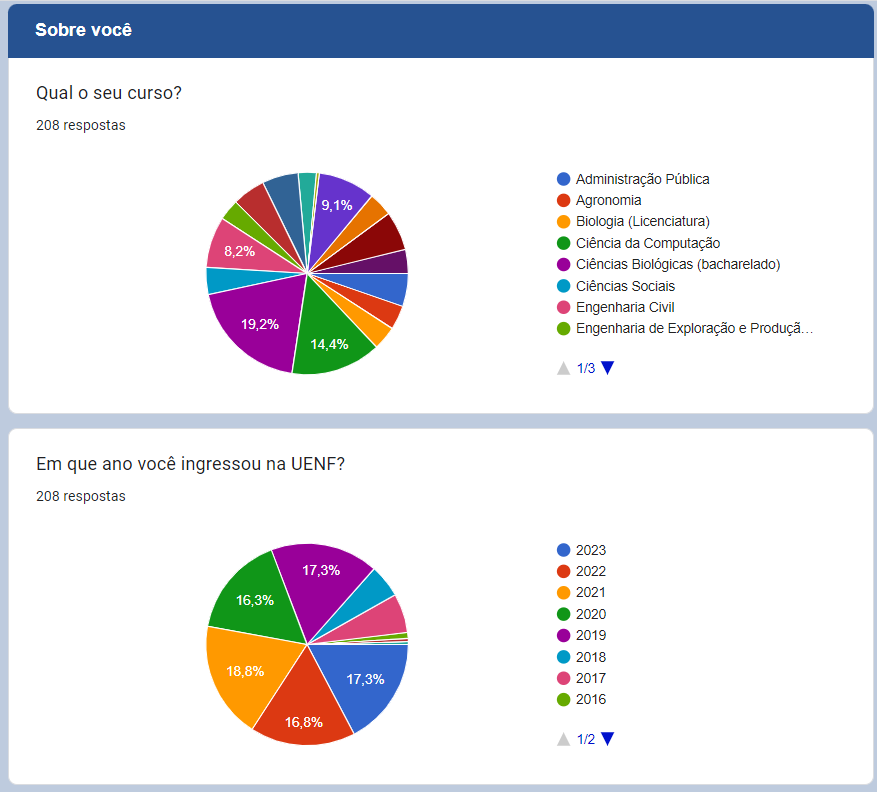
\includegraphics[width=\textwidth]{files/img/2.02!3-organizacao/2.02!3.1.4-forms/2.0-SobreVoce}
  % \end{MyCenteredFigure}

  O formulário foi respondido por 207 alunos, sendo os cursos de maior incidência o bacharelado de Ciências Biológicas com 40 respondentes, Ciência da Computação com 29 e Medicina Veterinária com 19. Vale ressaltar que 96 dos respondentes são alunos de cursos que envolvem diretamente o CCT. Entretanto, a análise dos gráficos abordará a percepção de todos igualmente.

  Vemos também a distribuição dos anos de ingresso dos alunos que responderam o formulário (\autoref{table:2.2_SobreVoce_Anos}), sendo seu quantitativo bem distribuído entre os anos de 2019 e 2023, tendo os anos de 2017 e 2018 uma quantidade menor de respostas, os outros anos tendo em conjunto um total de 4 respostas.

  \begin{CenteredTable} \caption{Número de respondentes por ano} \label{table:2.2_SobreVoce_Anos}
    \begin{tabular}{| c r c |}
      \hline
      \textbf{Quantidade} & \%   & \textbf{Ano} \\
      \hline
      36                  & 17,4 & 2023         \\
      35                  & 16,9 & 2022         \\
      39                  & 18,8 & 2021         \\
      34                  & 16,4 & 2020         \\
      35                  & 16,9 & 2019         \\
      11                  & 5,3  & 2018         \\
      13                  & 6,3  & 2017         \\
      2                   & 1,0  & 2016         \\
      1                   & 0,5  & 2015         \\
      0                   & 0,0  & 2014         \\
      0                   & 0,0  & 2013         \\
      1                   & 0,5  & Outro        \\
      \hline
    \end{tabular}
  \end{CenteredTable}

  \section*{Avaliação de experiência acadêmica} \label{sec:Avaliação de experiência acadêmica}

  Considerando que o escopo deste trabalho gira em torno da alocação de recursos físicos e humanos, como salas, professores e alunos, foi elaborada uma seção do formulário de pesquisa com o intuito de se analisar a frequência de ocorrência de certas situações no contexto universitário. Para isto, foram feitas as sete perguntas listadas a seguir.

  \begin{enumerate}
    \item \textbf{Salas}: você já teve que mudar de sala por falta de algum acessório como quadro, projetor ou monitor? % 53.1%
    \item \textbf{Salas}: você já teve aula cuja sala não dispunha de carteiras o suficiente? % 52.7%
    \item \textbf{Vagas}: você já quis entrar em uma disciplina, mas ela não tinha vaga? % 85.0%
    \item \textbf{Vagas}: você já ficou acordado após meia-noite por medo de não ter vaga para as disciplinas que deseja cursar? % 91.3%
    \item \textbf{Conflitos}: você já deixou de se inscrever em uma disciplina por causa de conflito de horário? % 90.8%
    \item \textbf{Preferências}: você já preferiu não se inscrever em uma disciplina para cursá-la em outro momento mais oportuno? % 86.0%
    \item \textbf{Opiniões}: você acha que a universidade deveria oferecer horários diferentes para as disciplinas mais demandadas para evitar conflitos com outras? % 100.0%
  \end{enumerate}

  A enumeração das perguntas feitas se encontra representada com suas respectivas respostas na \autoref{table:3.0_satisfacao}.

  \begin{CenteredTable} \caption{Ocorrência de experiências acadêmicas} \label{table:3.0_satisfacao}
    \begin{tabular}{| c | c c c | r r r |}
      \hline
      \multicolumn{1}{|c|}{\multirow{2}{*}{Pergunta}} & \multicolumn{3}{c|}{Respostas} & \multicolumn{3}{c|}{Respostas (\%)}                                                                  \\
      \multicolumn{1}{|c|}{}                          & Sim                            & \multicolumn{1}{|c|}{Não}           & Outro & Sim (\%) & \multicolumn{1}{|c|}{Não (\%)} & Outro (\%) \\
      \hline
      1                                               & 110                            & 87                                  & 10    & 53,1     & 42,0                           & 4,8        \\ % 110/207=0.5314 =  53.1%
      2                                               & 109                            & 95                                  & 3     & 52,7     & 45,9                           & 1,4        \\ % 109/207=0.5265 =  52.7%
      3                                               & 176                            & 28                                  & 3     & 85,0     & 13,5                           & 1,4        \\ % 176/207=0.8502 =  85.0%
      4                                               & 189                            & 17                                  & 1     & 91,3     & 8,2                            & 0,5        \\ % 189/207=0.9130 =  91.3%
      5                                               & 188                            & 15                                  & 4     & 90,8     & 7,2                            & 1,9        \\ % 188/207=0.9082 =  90.8%
      6                                               & 178                            & 27                                  & 2     & 86,0     & 13,0                           & 1,0        \\ % 178/207=0.8599 =  86.0%
      7                                               & 207                            & 0                                   & 0     & 100,0    & 0,0                            & 0,0        \\ % 207/207=1.0000 = 100.0%
      \hline
    \end{tabular}
  \end{CenteredTable}

  % \begin{MyCenteredFigure} \caption{Respostas sobre a satisfação dos estudantes} \label{fig:3.0_Satisfacao}
  %   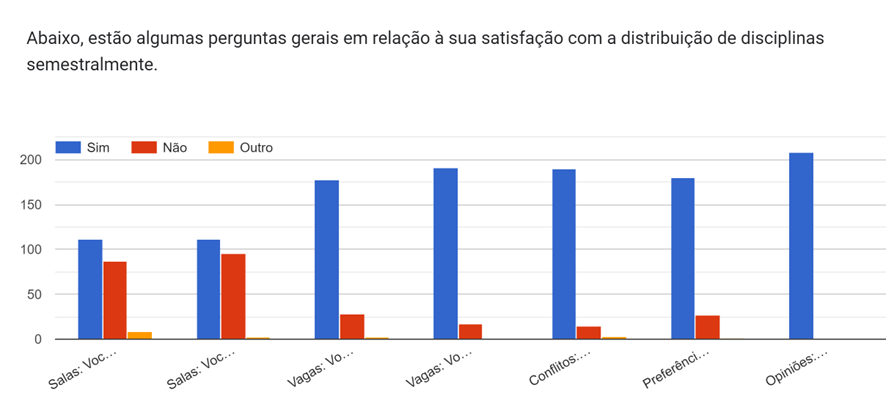
\includegraphics[width=\textwidth]{files/img/2.02!3-organizacao/2.02!3.1.4-forms/3.0-Satisfacao}
  % \end{MyCenteredFigure}

  Quanto à distribuição dos recursos físicos, vemos uma taxa de 53,1\% de alunos que já tiveram que mudar de sala por falta de algum acessório disposto necessário para a aula. Já a necessidade de mudança de sala devido à ausência de carteiras suficientes obteve taxa de 52,7\%.

  É notório o receio dos alunos quanto à possibilidade de não conseguir se inscrever nas disciplinas que desejam cursar, tendo sido confirmado por 85,0\% dos respondentes que se viram em situação em que a disciplina na qual desejavam se matricular não dispunha de vagas o bastante. Essa realidade resulta no temor por semestralmente não conseguir se inscrever na disciplina desejada, fazendo com que 91,3\% dos respondentes tenham se mantido acordados após a meia-noite por causa deste medo.

  O temor de não conseguir se inscrever nas disciplinas desejadas é ainda agravado pelo fato de que 90,8\% dos alunos que já deixaram de se inscrever em disciplinas devido a conflitos de horário.

  O que se apresenta como um agravante ainda maior na percepção da progressão não sequencial dos alunos é a quantidade de alunos que já preferiram não se inscrever em uma disciplina para cursá-la em outro momento mais oportuno, mesmo que isto signifique um atraso na progressão do curso, sendo seu percentual 86,0\%.

  Embora seja uma prática recorrente a oferta de diversas turmas para uma mesma disciplina, o que usualmente é feito de forma que as turmas sejam ofertadas no mesmo horário. Entretanto, os alunos, unanimemente, não se mostram satisfeitos com esta prática, visto que 100\% dos respondentes consideram que a universidade deveria dispor de outros horários para as disciplinas mais demandadas com o intuito de evitar conflitos de horários.

  Este resultado é curioso, visto que o temor de não se atrasar em seu progresso e conseguir se inscrever nas disciplinas desejadas, contrasta diretamente com a preferência pessoal de não se inscrever em disciplinas e cursá-las posteriormente, mesmo que isso possa atrasar seu progresso. Entende-se que nem todas as disciplinas, caso não cursadas em seu período esperado, resultarão no atraso da grade, mas ainda assim, a antítese é evidente.

  \section*{Preferências pessoais} \label{sec:Preferências pessoais}

  Neste segmento, visa-se entender um pouco melhor o processo decisório dos alunos quanto à escolha das disciplinas que desejam cursar. Primeiro, lhes é indagado quanto à disposição das disciplinas, variando entre disciplinas concentradas em poucos dias ou espalhadas durante a semana e quanto à preferência de horários, variando entre horários matutinos e vespertinos.

  Embora não lide com conflitos, a análise de seus resultados pode auxiliar na escolha de distribuição futura dos usuários do sistema, ao desenvolverem a grade horária, caso desejem considerar as preferências dos estudantes.

  \begin{comment}
  \begin{MyCenteredFigure} \caption{Preferências por distribuição de disciplinas ao longo da semana} \label{fig:4.1-PreferenciasPessoais-Distribuida_Acumulada}
    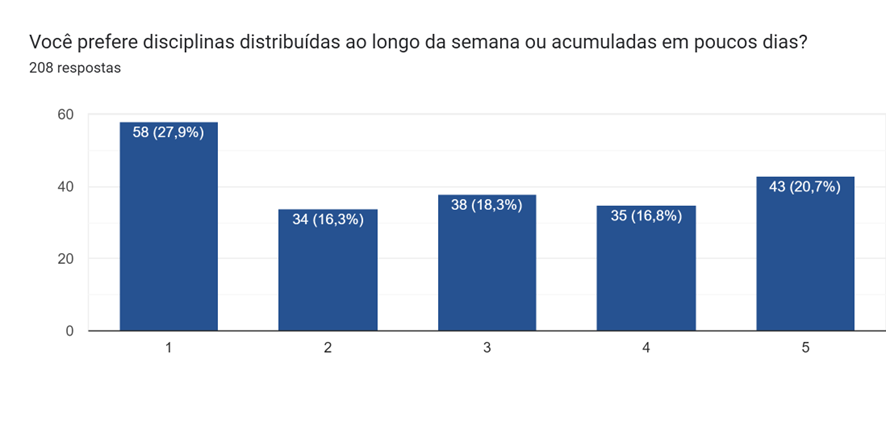
\includegraphics[width=\textwidth]{files/img/2.02!3-organizacao/2.02!3.1.4-forms/4.1-PreferenciasPessoais-Distribuida_Acumulada}
  \end{MyCenteredFigure}

  \begin{MyCenteredFigure} \caption{Preferências por distribuição de disciplinas em um mesmo dia} \label{fig:4.2-PreferenciasPessoais-Manha_Tarde}
    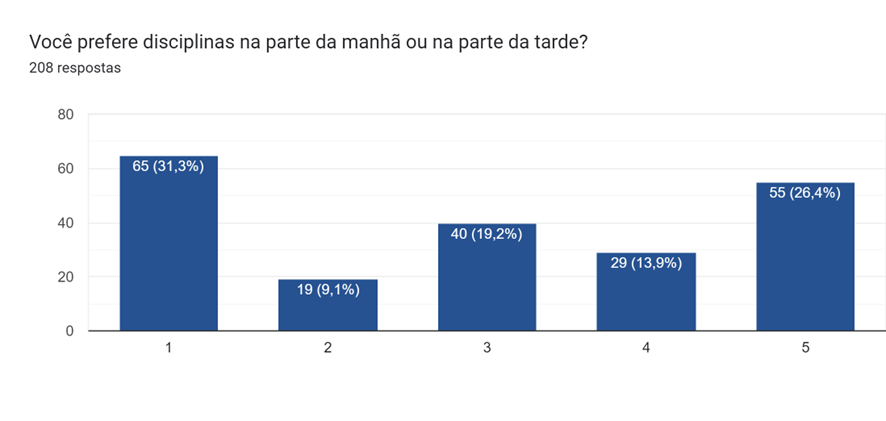
\includegraphics[width=\textwidth]{files/img/2.02!3-organizacao/2.02!3.1.4-forms/4.2-PreferenciasPessoais-Manha_Tarde}
  \end{MyCenteredFigure}
  \end{comment}

  Podemos ver na \autoref{table:4.1-PreferenciasPessoais-Distribuída_Acumulada} que há uma grande distribuição entre as preferências dos alunos, tendendo às extremidades, onde alguns preferem bastante as disciplinas distribuídas ao longo da semana enquanto outros preferem disciplinas acumuladas em poucos dias, vindo como terceira opção mais votada a neutralidade. Observação similar se mostra presente também na \autoref{table:4.2-PreferenciasPessoais-Manha_Tarde}.

  \begin{CenteredTable} \caption{Preferências por distribuição de disciplinas em um mesmo dia} \label{table:4.1-PreferenciasPessoais-Distribuída_Acumulada}
    \begin{tabular}{| r r l |}
      \hline
      \textbf{Quantidade} & \%   & \textbf{Distribuição na semana}            \\
      \hline
      58                  & 28,0 & Distribuídas ao longo da semana            \\
      34                  & 16,4 & Preferencialmente ao longo da semana       \\
      38                  & 18,4 & Não tenho preferência                      \\
      35                  & 16,9 & Preferencialmente acumulada em poucos dias \\
      42                  & 20,3 & Acumuladas em poucos dias                  \\
      \hline
    \end{tabular}
  \end{CenteredTable}

  \begin{CenteredTable} \caption{Preferências por distribuição de disciplinas em um mesmo dia} \label{table:4.2-PreferenciasPessoais-Manha_Tarde}
    \begin{tabular}{| r r l |}
      \hline
      \textbf{Quantidade} & \%   & \textbf{Distribuição no dia}        \\
      \hline
      65                  & 31,4 & Na parte da manhã                   \\
      19                  & 9,2  & Preferencialmente na parte da manhã \\
      40                  & 19,3 & Não tenho preferência               \\
      28                  & 13,5 & Preferencialmente na parte da tarde \\
      55                  & 26,6 & Na parte da tarde                   \\
      \hline
    \end{tabular}
  \end{CenteredTable}

  Em seguida, é questionado sobre qual é o critério de seleção de disciplinas que se apresentam conflituosas (\autoref{table:4.3-PreferenciasPessoais-Conflitos}). Nesta vertente vemos uma maior propensão à escolha por disciplinas que são pré-requisito de uma grande quantidade de disciplinas, ou seja, disciplinas que, caso se tenham reprovação ou não sejam cursadas, resultam no que é coloquialmente chamado de ``prender disciplinas'', assim atrasando mais a progressão do aluno. Sendo este o critério adotado por 81,6\% dos respondentes. A segunda maior opção selecionada foi a de escolher a disciplina mais concorrida, ou seja, a disciplina que possui uma maior demanda de alunos, sendo um critério utilizado por 25,1\% dos alunos.

  % \begin{MyCenteredFigure} \caption{Critérios para a escolha de disciplinas conflituosas} \label{fig:4.3-PreferenciasPessoais-Conflitos}
  %   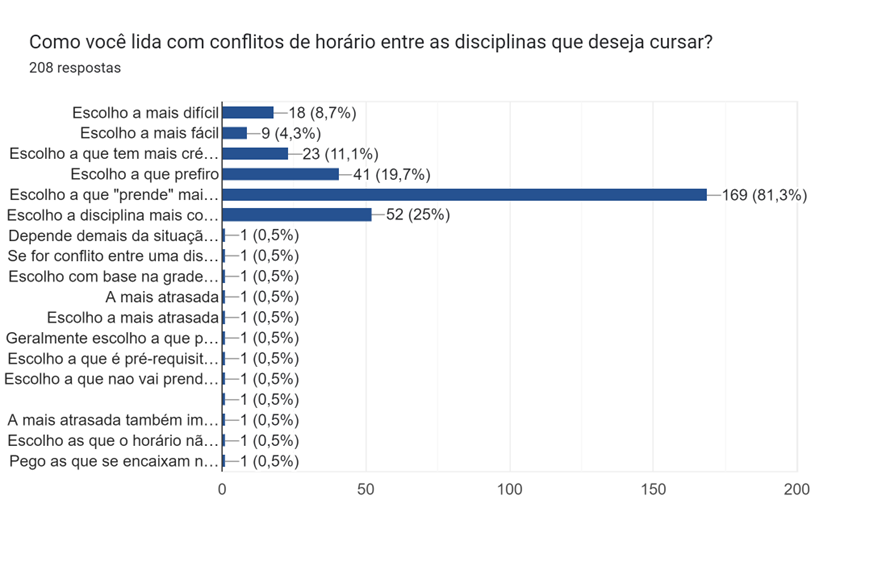
\includegraphics[width=\textwidth]{files/img/2.02!3-organizacao/2.02!3.1.4-forms/4.3-PreferenciasPessoais-Conflitos}
  % \end{MyCenteredFigure}

  \begin{CenteredTable} \caption{Critérios para a escolha de disciplinas conflituosas} \label{table:4.3-PreferenciasPessoais-Conflitos}
    \begin{tabular}{| r r l |}
      \hline
      \textbf{Quantidade} & \%   & \textbf{Forma de escolher disciplina conflituosa} \\
      \hline
      169                 & 81,6 & Escolho a que ``prende'' mais matérias            \\
      52                  & 25,1 & Escolho a disciplina mais concorrida              \\
      41                  & 19,8 & Escolho a que prefiro                             \\
      23                  & 11,1 & Escolho a que tem mais créditos                   \\
      18                  & 8,7  & Escolho a mais difícil                            \\
      12                  & 5,8  & Outro                                             \\
      9                   & 4,3  & Escolho a mais fácil                              \\
      \hline
    \end{tabular}
  \end{CenteredTable}

  Vale ressaltar que as respostas ilustradas pela \autoref{table:4.3-PreferenciasPessoais-Conflitos} permite a seleção de múltiplas escolhas, inclusive permitindo que adicionassem outros critérios próprios. Dentre eles, um se mostrou ligeiramente recorrente que seria escolher a disciplina mais atrasada segundo a grade curricular. Outra possibilidade citada foi selecionar a que se encaixam na disponibilidade de horário pessoal, para que não conflite, por exemplo, com o horário do estágio obrigatório.

  \section*{Experiências com atrasos e disciplinas} \label{sec:Experiências com atrasos e disciplinas}

  Quanto aos atrasos para a realização de disciplinas, o ideal desejado é que não haja nenhum atraso. Nessa situação, todos os alunos que entram na universidade poderão seguir a disponibilidade usual das disciplinas dispostas em suas grades curriculares, que apresentam o período esperado para que cada disciplina seja realizada. Sendo elas, usualmente dividas como disciplinas pares e ímpares. As ímpares se referem às disciplinas em que se espera que sejam cursadas nos períodos 1, 3, 5, 7 e 9, e que são ofertadas no primeiro semestre letivo. Enquanto que as pares se referem às disciplinas oferecidas no segundo período letivo, onde geralmente se alocam as disciplinas dos períodos 2, 4, 6, 8 e 10.

  Entretanto, a realidade dos alunos é outra. Isso se dá por diversos motivos, seja por reprovação, por não conseguir se inscrever na disciplina desejada ou por simplesmente não ter interesse em cursar a disciplina naquele momento, como já ilustrado na \autoref{table:3.0_satisfacao}. Esta característica se confirma na percepção da frequência e distância que percebemos dos atrasos, representado pela \autoref{table:5.0-Atrasos}.
  Períodos de atraso

  \begin{enumerate}
    \item Quanto tempo (em períodos) você já teve que esperar para fazer uma disciplina da sua grade?
    \item Qual foi a quantidade máxima de períodos que você se distanciou de uma disciplina de determinado período?
  \end{enumerate}

  \begin{CenteredTable} \caption{Tempo de atraso em disciplinas} \label{table:5.0-Atrasos}
    \begin{tabular}{| c | c c c c c c c c c c c |}
      \hline
      \multicolumn{1}{|c|}{\multirow{2}{*}{Pergunta}} &
      \multicolumn{11}{c|}{Períodos de atraso}                                                                               \\
      \multicolumn{1}{|c|}{}                          &
      \multicolumn{1}{c|}{0}                          &
      \multicolumn{1}{c|}{1}                          &
      \multicolumn{1}{c|}{2}                          &
      \multicolumn{1}{c|}{3}                          &
      \multicolumn{1}{c|}{4}                          &
      \multicolumn{1}{c|}{5}                          &
      \multicolumn{1}{c|}{6}                          &
      \multicolumn{1}{c|}{7}                          &
      \multicolumn{1}{c|}{8}                          &
      \multicolumn{1}{c|}{9}                          &
      \multicolumn{1}{|c|}{10}
      \\
      \hline
      1                                               & 53   & 38   & 79   & 19   & 11   & 1   & 1   & 3   & 1   & 1   & 0   \\
      2                                               & 33   & 27   & 60   & 31   & 28   & 15  & 9   & 1   & 2   & 1   & 0   \\
      \hline
      1 (\%)                                          & 25,6 & 18,4 & 38,2 & 9,2  & 5,3  & 0,5 & 0,5 & 1,4 & 0,5 & 0,5 & 0,0 \\
      2 (\%)                                          & 15,9 & 13,0 & 29,0 & 15,0 & 13,5 & 7,2 & 4,3 & 0,5 & 1,0 & 0,5 & 0,0 \\
      \hline
    \end{tabular}
  \end{CenteredTable}

  \begin{comment}
  \begin{MyCenteredFigure} \caption{Períodos de atraso por espera} \label{fig:5.1-Atrasos-Esperar}
    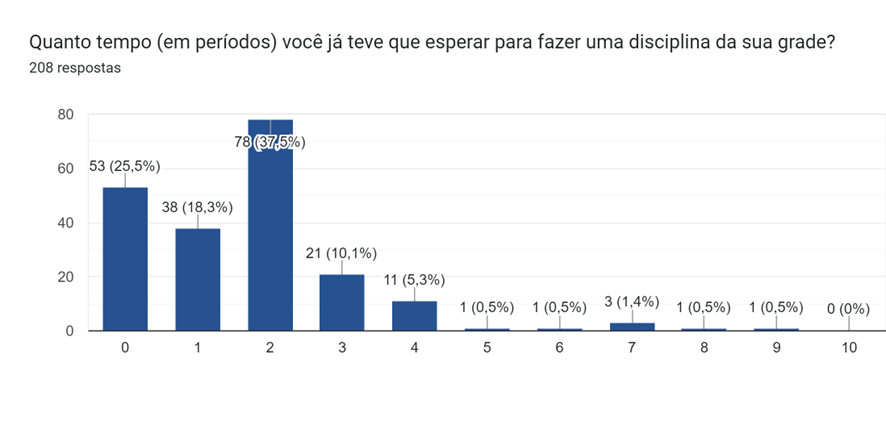
\includegraphics[width=\textwidth]{files/img/2.02!3-organizacao/2.02!3.1.4-forms/5.1-Atrasos-Esperar}
  \end{MyCenteredFigure}

  \begin{MyCenteredFigure} \caption{Distância de atraso} \label{fig:5.2-Atrasos-Distancia}
    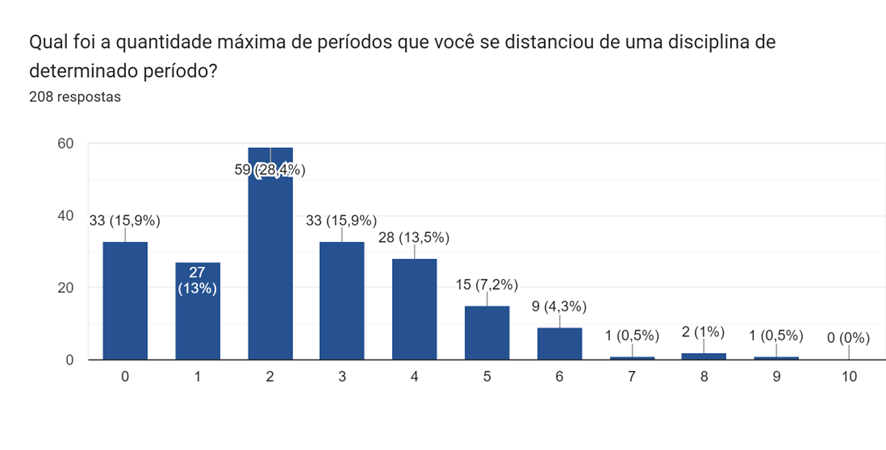
\includegraphics[width=\textwidth]{files/img/2.02!3-organizacao/2.02!3.1.4-forms/5.2-Atrasos-Distancia}
  \end{MyCenteredFigure}
  \end{comment}

  Apresenta-se notável que é minoria a quantidade de alunos que nunca tiveram que esperar para cursar uma disciplina, sendo estes apenas 25,6\% dos respondentes. É ainda mais notável o fato de que o tempo de espera médio é de mais de um semestre. Quanto ao distanciamento de disciplinas, seja por reprovações ou por escolha própria se mostra ainda mais presente, sendo que apenas 15,9\% dos respondentes não se distanciaram das disciplinas esperadas para o período, sendo o tempo médio de distanciamento maior que dois semestres.

  \section*{Pesquisa de opinião} \label{sec:Pesquisa de opinião}

  Aqui, busca-se uma análise mais bruta e direta à concordância dos respondentes quanto às características atribuídas à distribuição de disciplinas semestrais, ondem eles avaliam com notas de 1 a 5 o quanto concordam com cada uma das características dadas à distribuição de disciplinas, sendo eles ``Justa'' (feita de acordo a atender os desejos da maioria), ``Variada'' (bem diversa e abrange diversos interesses), ``Contínua'' (oferecida de forma a ter aulas sequenciais), ``Eficiente'' (bem sucedida em atender aos desejos dos alunos), ``Distribuída'' (bem espaçada ao longo da semana) e ``Satisfatória'' (agradável aos meus desejos pessoais). Estando as opiniões dos alunos refletidas nos resultados expostos pela \autoref{table:6.0-Opiniao}, seguidas das médias por característica.

  \begin{CenteredTable} \caption{Notas dadas às características da distribuição de disciplinas} \label{table:6.0-Opiniao}
    \begin{tabular}{| l | c c c c c | c |}
      \hline
      \multicolumn{1}{|c|}{\multirow{2}{*}{Opções}} &
      \multicolumn{5}{c|}{Notas}                    &
      \multicolumn{1}{c|}{\multirow{2}{*}{Médias}}
      \\
      \multicolumn{1}{|c|}{}                        &
      \multicolumn{1}{c|}{1}                        &
      \multicolumn{1}{c|}{2}                        &
      \multicolumn{1}{c|}{3}                        &
      \multicolumn{1}{c|}{4}                        &
      \multicolumn{1}{c|}{5}                        &
      \multicolumn{1}{c|}{}                                                        \\
      \hline
      Justa                                         & 59 & 69 & 52 & 17 & 10 & 2,3 \\
      Variada                                       & 40 & 65 & 64 & 26 & 12 & 2,5 \\
      Contínua                                      & 34 & 44 & 78 & 41 & 10 & 2,8 \\
      Eficiente                                     & 61 & 76 & 45 & 17 & 8  & 2,2 \\
      Distribuída                                   & 32 & 40 & 61 & 60 & 14 & 2,9 \\
      Satisfatória                                  & 40 & 61 & 68 & 30 & 8  & 2,5 \\
      \hline
    \end{tabular}
  \end{CenteredTable}

  \begin{comment}
  \begin{MyCenteredFigure} \caption{Notas dadas para as características da distribuição de disciplinas} \label{fig:6.0-Opiniao-Todas}
    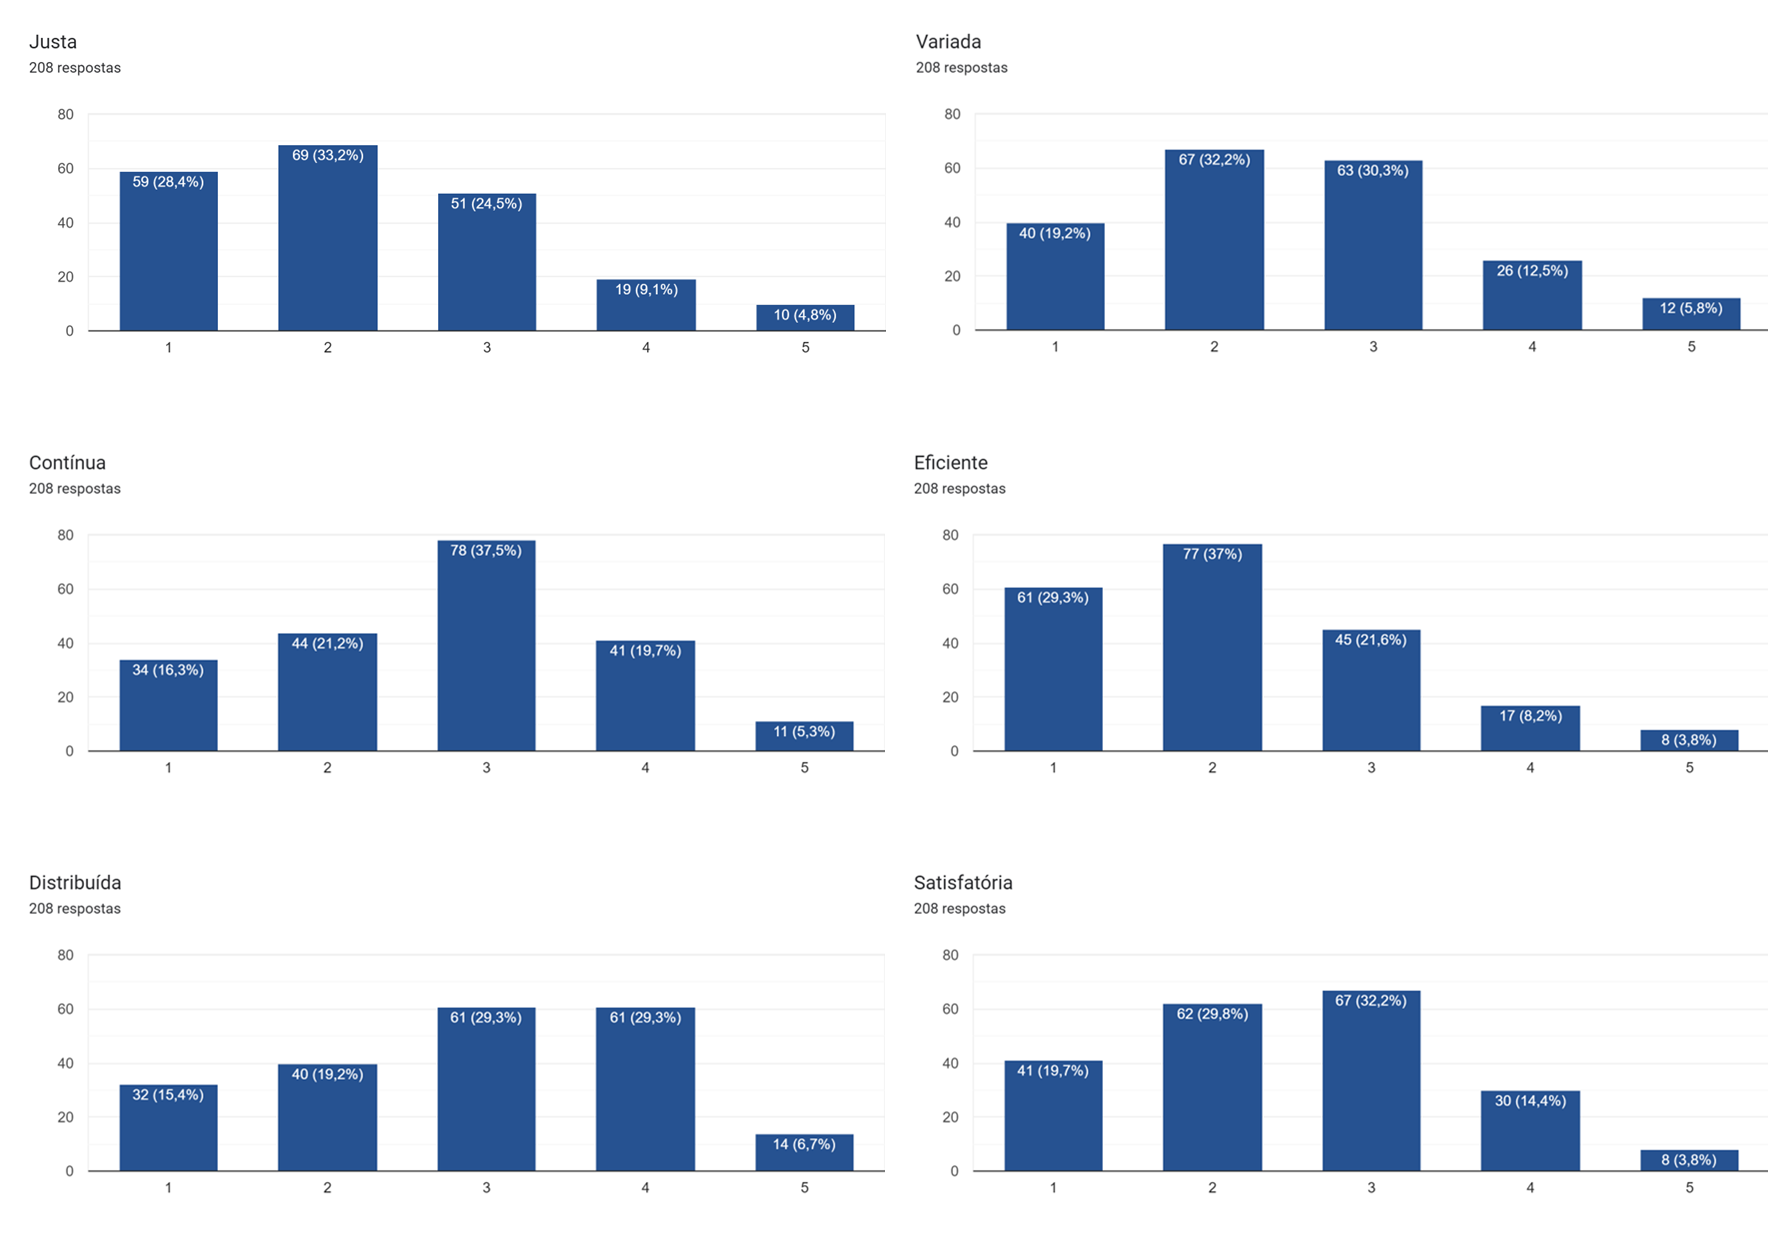
\includegraphics[width=\textwidth]{files/img/2.02!3-organizacao/2.02!3.1.4-forms/6.0-Opiniao-Todas}
  \end{MyCenteredFigure}

  \begin{MyCenteredFigure} \caption{Resultados das características ``Justa'', ``Variada'' e ``Contínua''} \label{fig:6.0-Opiniao-1_3}
    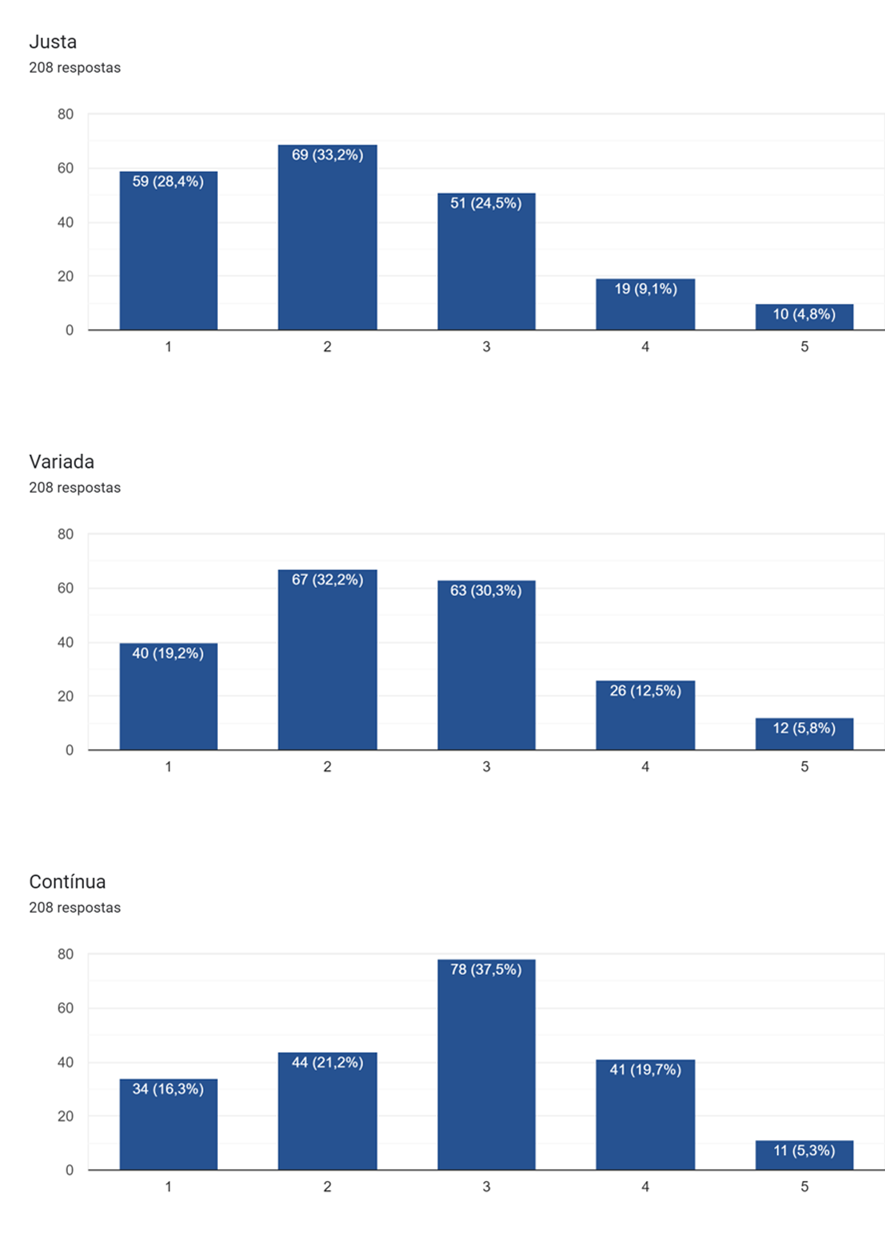
\includegraphics[width=\textwidth]{files/img/2.02!3-organizacao/2.02!3.1.4-forms/6.0-Opiniao-1_3}
  \end{MyCenteredFigure}

  \begin{MyCenteredFigure} \caption{Resultados das características ``Eficiente'', ``Distribuída'' e ``Satisfatória''} \label{fig:6.0-Opiniao-4_6}
    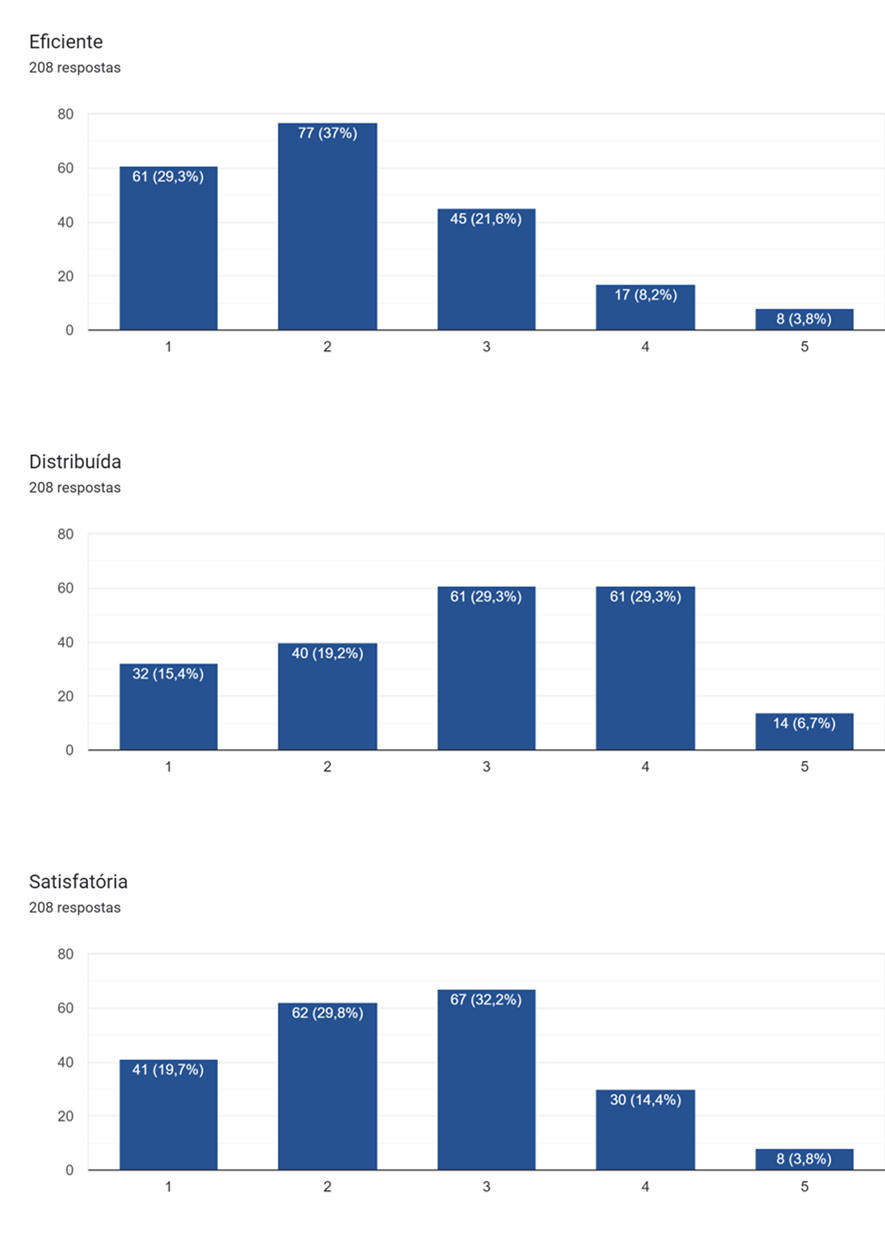
\includegraphics[width=\textwidth]{files/img/2.02!3-organizacao/2.02!3.1.4-forms/6.0-Opiniao-4_6}
  \end{MyCenteredFigure}

  \begin{MyCenteredFigure} \caption{Notas dadas para a característica: justa} \label{fig:6.1-Opiniao-Justa}
    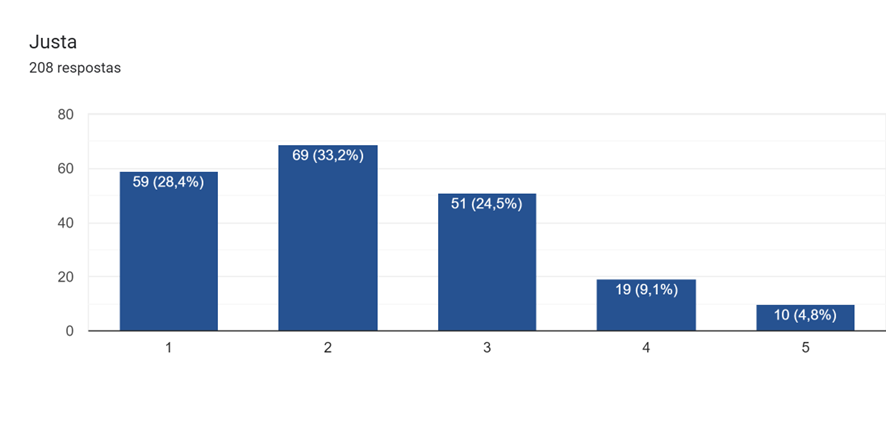
\includegraphics[width=\textwidth]{files/img/2.02!3-organizacao/2.02!3.1.4-forms/6.1-Opiniao-Justa}
  \end{MyCenteredFigure}

  \begin{MyCenteredFigure} \caption{Notas dadas para a característica: variada} \label{fig:6.2-Opiniao-Variada}
    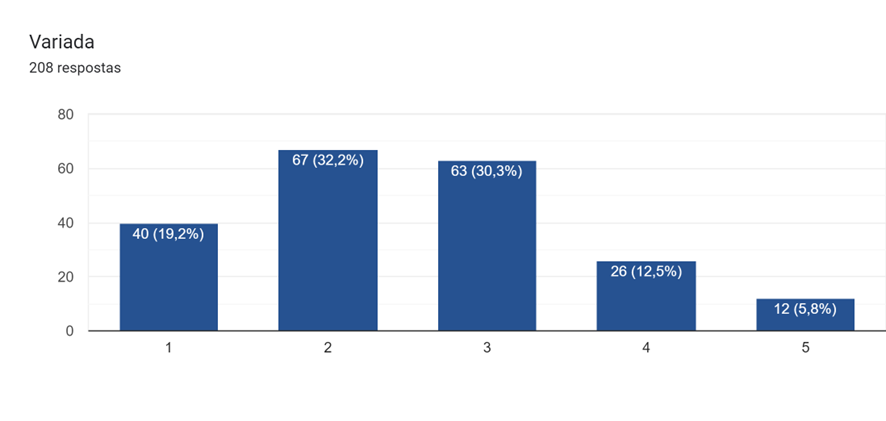
\includegraphics[width=\textwidth]{files/img/2.02!3-organizacao/2.02!3.1.4-forms/6.2-Opiniao-Variada}
  \end{MyCenteredFigure}

  \begin{MyCenteredFigure} \caption{Notas dadas para a característica: contínua} \label{fig:6.3-Opiniao-Continua}
    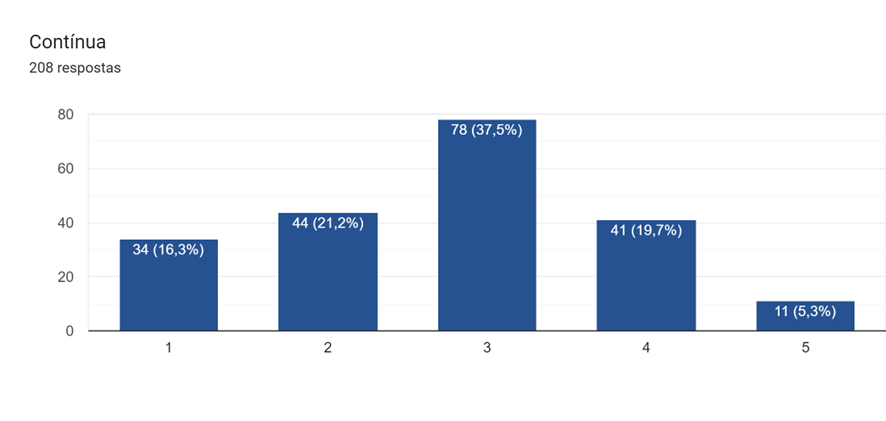
\includegraphics[width=\textwidth]{files/img/2.02!3-organizacao/2.02!3.1.4-forms/6.3-Opiniao-Continua}
  \end{MyCenteredFigure}

  \begin{MyCenteredFigure} \caption{Notas dadas para a característica: eficiente} \label{fig:6.4-Opiniao-Eficiente}
    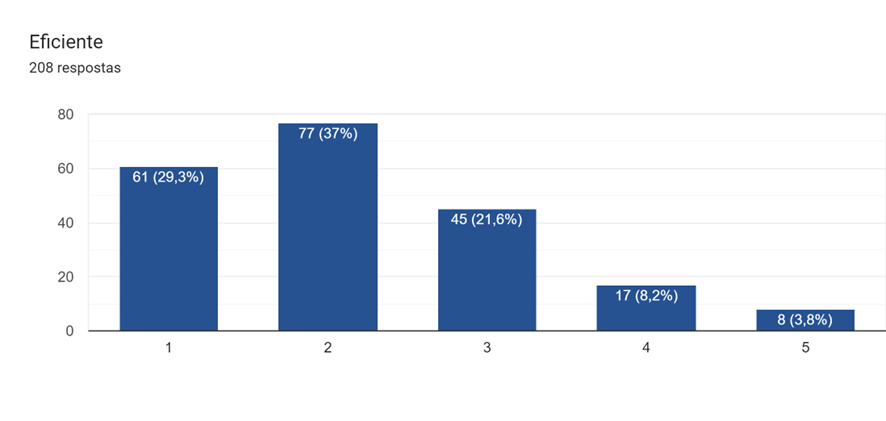
\includegraphics[width=\textwidth]{files/img/2.02!3-organizacao/2.02!3.1.4-forms/6.4-Opiniao-Eficiente}
  \end{MyCenteredFigure}

  \begin{MyCenteredFigure} \caption{Notas dadas para a característica: distribuída} \label{fig:6.5-Opiniao-Distribuida}
    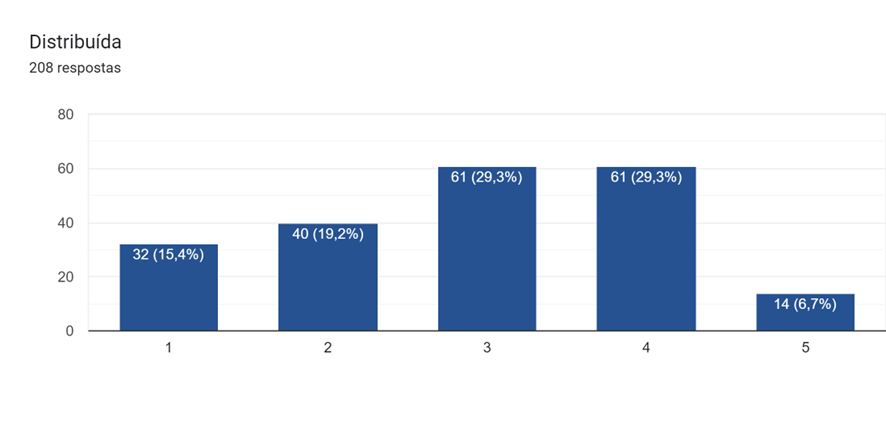
\includegraphics[width=\textwidth]{files/img/2.02!3-organizacao/2.02!3.1.4-forms/6.5-Opiniao-Distribuida}
  \end{MyCenteredFigure}

  \begin{MyCenteredFigure} \caption{Notas dadas para a característica: satisfatória} \label{fig:6.6-Opiniao-Satisfatoria}
    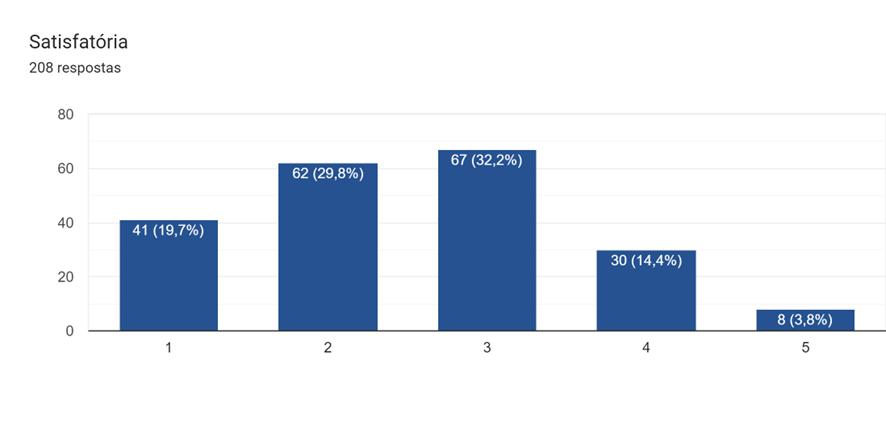
\includegraphics[width=\textwidth]{files/img/2.02!3-organizacao/2.02!3.1.4-forms/6.6-Opiniao-Satisfatoria}
  \end{MyCenteredFigure}
  \end{comment}

  De uma forma geral, conseguimos ver todos os gráficos com menos de 7\% dos respondentes dando nota 5 em cada uma das características, A maioria das respostas tende a estar entre 1 e 3, sendo exceção apenas no caso da característica ``distribuída'', que por sua vez apresenta uma elevada quantidade de notas 4, sendo referente a 29,3\% dos respondentes.

  Ao analisarmos a média de cada uma, podemos dizer que, em suma, há o visível desagrado do corpo discente quanto à distribuição de disciplinas semestrais, com ênfase nas duas piores notas que são 2,2 para ``eficiente'' e 2,3 para ``justa'' o que reforça a necessidade de aprimoramento do sistema atual.

  \section*{Respostas qualitativas} \label{sec:Respostas qualitativas}

  Por fim, havia um espaço livre no formulário para que os alunos pudessem expressar suas opiniões de forma mais livre. Após a leitura de todas e a filtragem das opiniões expressas, resumem-se em 4 parabenizações pelo desenvolvimento do presente projeto, 18 reclamações e 16 sugestões. Dentre elas, algumas apresentaram maior recorrência, sendo elas:

  \begin{itemize}
    \item 5 reclamações sobre a usual oferta de disciplinas separadas entre pares e ímpares;
    \item 4 reclamações sobre o Sistema Acadêmico, principalmente sobre não ser capaz de suportar a carga nos momentos iniciais de inscrição de disciplinas;
    \item 3 sugestões de ofertas de disciplinas recorrentemente, com ênfase nas disciplinas de matemática/que contemplam diversos cursos/com alta taxa de reprovação;
    \item 3 sugestões de mais oferta de disciplinas no período de verão;
    \item 2 sugestões de que inscrições em matérias do semestre atual esperado do aluno fossem feitas automaticamente, mas ainda permitindo a sua exclusão caso desejado;
    \item 1 sugestão de criação de um formulário de demanda no acadêmico que computasse a intenção de matrícula dos alunos.
  \end{itemize}

  Abaixo estão dispostas algumas das respostas obtidas:

  \begin{itemize}
    \item ``A estrutura curricular deveria ser predefinida, automatizando a matrícula dos alunos nas disciplinas correspondentes aos seus períodos acadêmicos. No entanto, permitir-se-ia a edição do cronograma por parte dos alunos, caso desejem quitar pendências de períodos anteriores ou disciplinas antecipadas. Além disso, disciplinas que abrangem múltiplos cursos devem ser oferecidas em ambos os semestres.

          Para melhorar a oferta de disciplinas, seria aconselhável ampliar a disponibilidade de disciplinas durante o período de verão. Isso facilitaria o acesso dos alunos ao estágio obrigatório durante as férias, viabilizando a conclusão dessa etapa essencial do curso.
            % Reduzir o número de créditos necessários para antecipar a realização do estágio também se mostraria benéfico, visto que atualmente, a conclusão dessa matéria com apenas 9 créditos pendentes inviabiliza a possibilidade de antecipação antes do 9º período. Considera-se viável permitir essa antecipação a partir do 7º período.
            [...] Essas melhorias no sistema acadêmico [...] agilizariam a trajetória do estudante, permitindo maior flexibilidade na escolha e realização de disciplinas [...].''
    \item ``Existe muita desorganização em relação a grade, disciplinas e sistema acadêmico por parte dos coordenadores dos cursos. Me inscrevi numa matéria que tinha requisito de acordo com o plano pedagógico, mas tanto na grade como no sistema acadêmico não tinha pré-requisito nenhum. Tive que desistir da matéria pela dificuldade, até porque a matéria que era pré-requisito eu perdi. Detalhe: Outras pessoas perderam na matéria pré-requisito e continuaram fazendo a matéria desse período.''
    \item ``Acho que as coordenações precisam estabelecer um melhor diálogo com os alunos. Esse sistema de período par e ímpar na UENF é antigo e perpetua um comodismo dos professores que acabam não ofertando disciplinas todos os semestres e prejudicando os alunos nas escolhas de matérias optativas, eletivas, instrumentais e obrigatórias tendo que esperar um ano para realizar a disciplina caso você não consiga fazer por choque de horário e/ou reprovação.''
  \end{itemize}

  \section*{Conclusões} \label{sec:Conclusões}

  Por fim, entendemos que, além das insatisfações dormentes por parte dos gestores e criadores de grades horárias, os alunos também se mostram insatisfeitos com a atual estrutura de distribuição de disciplinas semestrais. Os interesses dos alunos se mostram em sua maioria alinhados com os interesses dos gestores, onde ambos visam reduzir a quantidade de atrasos na progressão do curso.

  \chapter{Código-Fonte da Monografia} \label{apendice:CodigoFonte}

  Como forma mais prática é sugerida de acesso ao código-fonte da monografia, recomenda-se acessar o \LinkToURL{\LinkCodigoFonteSistema}{repositório do GitHub}, nele constará o código-fonte mais atualizado do sistema. Caso por algum motivo o link não esteja funcionando apropriadamente, está disponibilizado também na guia de Anexos do documento PDF deste trabalho o código-fonte do sistema. Para acessá-lo, basta procurar a aba de anexos em algum leitor de PDF que suporte anexos, como por exemplo o \LinkToURL{\LinkAdobeReader}{Adobe Reader}, ou clique
  \textattachfile{files/codigos/CodigoFonteSistema.rar.RemovaEstaParteParaAcessarOCodigo}{aqui}.

  Além do código do sistema, também está disponível o código-fonte \LaTeX deste documento, também num \LinkToURL{\LinkCodigoFonteMonografia}{repositório do GitHub}, porém nesse caso, talvez seja necessário passar por uma burocracia antes, visto que o primeiro link é de um repositório contido em uma organização privada, sendo necessário primeiro obter acesso a ela através de um procedimento descrito \LinkToURL{\LinkDisciplinas}{aqui}. Caso prefira, assim como no caso anterior, dispõe-se também o código-fonte \LaTeX deste documento na guia de Anexos do documento PDF, ou clique
  \textattachfile{files/codigos/CodigoFonteLaTeX.rar.RemovaEstaParteParaAcessarOCodigo}{aqui}.

  Como em alguns casos o leitor de PDF pode não ter suporte para abrir arquivos compactados, a extensão do arquivo foi alterada. Para acessar o arquivo, basta salvá-lo em seu computador, remover a parte final do nome do arquivo e descompactá-lo utilizando um programa de sua preferência. Caso prefira, também é possível abrir o arquivo diretamente com o programa de compactação, sem a necessidade de alterar o nome.

  \chapter{Formulário de pesquisa editável} \label{apendice:FormularioPesquisaQuantitativaEditavel}

  Abaixo está o formulário de pesquisa quantitativa de alunos da UENF sobre distribuição e oferta de disciplinas. Este formulário foi feito em \LaTeX{} e é editável, podendo ser preenchido e enviado por e-mail. Para preenchê-lo, basta clicar no campo desejado e preencher com as informações solicitadas. Para enviar o formulário, clique no botão ``Enviar''.

  \begin{Form}[action=mailto:joaovitorfd2000@gmail.com, encoding=html, method=post]

    Pesquisa quantitativa de alunos da UENF sobre distribuição e oferta de disciplinas

    \section*{Pesquisa quantitativa de alunos da UENF sobre distribuição e oferta de disciplinas}

    Olá! Desde já agradeço por ceder em torno de 4 minutos do seu tempo para responder a este formulário usando o seu e-mail institucional. Considerando que nosso tempo é valioso, vamos direto ao objetivo:

    Me chamo João Vítor Fernandes Dias, estudante de Ciência da Computação na UENF, e estou fazendo minha Monografia. Ela trata da elaboração de um sistema para a coordenação de curso poder analisar mais facilmente quais são as disciplinas que serão disponibilizadas a cada semestre e a quais salas e professores serão atribuídas.

    O objetivo da minha monografia é conseguir tornar mais eficiente a distribuição das disciplinas, para que se resulte em um conjunto de disciplinas ofertadas com melhor qualidade. Espera-se com isso que as demandas de disciplina dos alunos sejam melhor atendidas, assim como as preferências de horários dos professores.

    Este formulário tem como objetivo avaliar a sua satisfação em relação ao processo de inscrição semestral nas disciplinas.

    \section*{Sobre você}

    Nesta seção, peço que informe algumas características suas para que a análise estatística se torne mais rica.

    \begin{enumerate}
      \QuestionNameOptions{Qual o seu curso?}{curso}
      {
        1. Administração Pública,
        2. Agronomia,
        3. Biologia (Licenciatura),
        4. Ciência da Computação,
        5. Ciências Biológicas (bacharelado),
        6. Ciências Sociais,
        7. Engenharia Civil,
        8. Engenharia de Exploração e Produção de Petróleo,
        9. Engenharia de Produção,
        10. Engenharia Metalúrgica,
        11. Engenharia Meteorológica,
        12. Física (licenciatura),
        13. Matemática (Licenciatura),
        14. Medicina Veterinária,
        15. Pedagogia (Licenciatura),
        16. Química (Licenciatura),
        17. Zootecnia,
        18. Outro,
      }
      \QuestionNameOptions{Em que ano você ingressou na UENF?}{anoIngresso}
      { 2023, 2022, 2021, 2020, 2019, 2018, 2017, 2016, 2015, 2014, 2013, Outro }
    \end{enumerate}

    \section*{Pesquisa de satisfação}

    Agora serão feitas algumas perguntas em relação à sua satisfação com algumas características da Universidade.

    Abaixo, estão algumas perguntas gerais em relação à sua satisfação com a distribuição de disciplinas semestralmente.

    \begin{enumerate}
      \ChoiceMenuSNO{\textbf{Salas}: Você já teve que mudar de sala por falta de algum acessório como quadro, projetor ou monitor?}{SalasAcessorios}
      \ChoiceMenuSNO{\textbf{Salas}: Você já teve aula cuja sala não dispunha de carteiras o suficiente?}{SalasCarteiras}
      \ChoiceMenuSNO{\textbf{Vagas}: Você já quis entrar em uma disciplina, mas ela não tinha vaga?}{VagasDisciplinas}
      \ChoiceMenuSNO{\textbf{Vagas}: Você já ficou acordado após meia-noite por medo de não ter vaga para as disciplinas que deseja cursar?}{VagasNoite}
      \ChoiceMenuSNO{\textbf{Conflitos}: Você já deixou de se inscrever em uma disciplina por causa de conflito de horário?}{Conflitos}
      \ChoiceMenuSNO{\textbf{Preferências}: Você já preferiu não se inscrever em uma disciplina para cursá-la em outro momento mais oportuno?}{Preferências}
      \ChoiceMenuSNO{\textbf{Opiniões}: Você acha que a universidade deveria oferecer horários diferentes para as disciplinas mais demandadas para evitar conflitos com outras disciplinas?}{Opiniões}
    \end{enumerate}

    \section*{Preferências pessoais}

    Esta seção visa saber um pouco mais sobre as suas preferências pessoais quanto a escolha das disciplinas ofertadas.

    \begin{enumerate}
      \item Você prefere disciplinas distribuídas ao longo da semana ou acumuladas em poucos dias?
            \FormInNewLine{
              \ChoiceMenu[print, combo, name=distribuiçãoDisciplinasNaSemana]{ }
              {
                1. Distribuídas ao longo da semana,
                2. Preferencialmente ao longo da semana,
                3. Não tenho preferência,
                4. Preferencialmente acumulada em poucos dias,
                5. Acumuladas em poucos dias,
              }
            }

      \item Você prefere disciplinas na parte da manhã ou na parte da tarde?
            \FormInNewLine{
              \ChoiceMenu[print, combo, name=distribuiçãoDisciplinasNoDia]{ }
              {
                1. Na parte da manhã,
                2. Preferencialmente na parte da manhã,
                3. Não tenho preferência,
                4. Preferencialmente na parte da tarde,
                5. Na parte da tarde,
              }

            }
      \item Como você lida com conflitos de horário entre as disciplinas que deseja cursar?
            \begin{itemize}
              \MyCheckbox{Escolho a mais difícil}{dificil}
              \MyCheckbox{Escolho a mais fácil}{facil}
              \MyCheckbox{Escolho a que tem mais créditos}{creditos}
              \MyCheckbox{Escolho a que prefiro}{prefiro}
              \MyCheckbox{Escolho a que ``prende'' mais matérias}{prende}
              \MyCheckbox{Escolho a disciplina mais concorrida}{concorrida}
              \item \TextField[name=ComentarioConflito, width=0.8\linewidth]{Outro...}
            \end{itemize}
    \end{enumerate}

    \section*{Experiências passadas com atrasos e disciplinas}

    Aqui estão algumas perguntas relacionadas à divergência entre o período esperado de conclusão das disciplinas VS o período em que elas de fato são realizadas.

    \begin{enumerate}
      \ChoiceMenuPeriodos{Quanto tempo (em períodos) você já teve que esperar para fazer uma disciplina da sua grade?}{TempoEspera}
      \ChoiceMenuPeriodos{Qual foi a quantidade máxima de períodos que você se distanciou de uma disciplina de determinado período?}{DistanciaPeriodos}
    \end{enumerate}

    \section*{Você acha que a distribuição de disciplinas semestrais é...}

    \begin{enumerate}
      \ChoiceMenuDdNcC{Justa (feita de acordo a atender os desejos da maioria)}{Justa}
      \ChoiceMenuDdNcC{Variada (bem diversa e abrange diversos interesses)}{Variada}
      \ChoiceMenuDdNcC{Contínua (oferecida de forma a ter aulas sequenciais)}{Contínua}
      \ChoiceMenuDdNcC{Eficiente (bem sucedida em atender aos desejos dos alunos)}{Eficiente}
      \ChoiceMenuDdNcC{Distribuída (bem espaçada ao longo da semana)}{Distribuída}
      \ChoiceMenuDdNcC{Satisfatória (agradável aos meus desejos pessoais)}{Satisfatória}
    \end{enumerate}

    \section*{Opcional}

    Por fim, deixo aqui um espaço caso deseje compartilhar algum comentário, opinião ou sugestão quanto ao meu trabalho ou formulário.

    Escreva aqui caso haja algo que gostaria de comentar, opinar ou sugerir. Tudo bem deixar em branco, suas informações já foram de grande ajuda.

    \TextField[multiline=true, width=0.8\linewidth, name=comentario]{ }

    \Reset{Resetar}
    \Submit{Enviar}

  \end{Form}





  \chapter{Exemplo de \textit{template.yaml}} \label{apendice:ExemploTemplateYAML}

  O arquivo \textit{template.yaml} é um arquivo de configuração do \textit{AWS SAM} que define como a aplicação será construída e como será feito o deploy dela. Abaixo está um exemplo deste arquivo.

  \lstinputlisting[language={YAML}, captionpos={t}, label={code:template}, caption={Exemplo de \textit{template.yaml}}]{files/codigos/AWS_SAM.yaml}

\end{apendicesenv}


\chapter*{56. Referências 1/4}
\chapter*{57. Referências 2/4}
\chapter*{58. Referências 3/4}
\chapter*{59. Referências 4/4}
\chapter*{60. Fim}

\end{document}
